%%% main.tex --- 
%% 
%% Filename: main.tex
%% Description: 
%% Author: Ola Leifler
%% Maintainer: 
%% Created: Thu Oct 14 12:52:20 2010 (CEST)
%% Version: $Id$
%% Version: 
%% Last-Updated: Wed Jun 28 10:57:24 2017 (+0200)
%%           By: Ola Leifler
%%     Update #: 169
%% URL: 
%% Keywords: 
%% Compatibility: 
%% 
%%%%%%%%%%%%%%%%%%%%%%%%%%%%%%%%%%%%%%%%%%%%%%%%%%%%%%%%%%%%%%%%%%%%%%
%% 
%%% Commentary: 
%% 
%% 
%% 
%%%%%%%%%%%%%%%%%%%%%%%%%%%%%%%%%%%%%%%%%%%%%%%%%%%%%%%%%%%%%%%%%%%%%%
%% 
%%% Change log:
%% 
%% 
%% RCS $Log$
%%%%%%%%%%%%%%%%%%%%%%%%%%%%%%%%%%%%%%%%%%%%%%%%%%%%%%%%%%%%%%%%%%%%%%
%% 
%%% Code:

\documentclass[msc,lith,english]{liuthesis}
%% Settings go in settings.tex
\include{settings}
\usepackage{rotating}
\usepackage{color}

% \usepackage{changebar}

\department{Institutionen för datavetenskap}
\departmentenglish{Department of Computer and Information Science}
\departmentshort{IDA}
% If this is a thesis at the cognitive science study programme, use
% the "area" command to generate a proper (?) ISRN
% \area{KOGVET-A}

% Include an external supervisor on the cover page
\externalsupervisor{Erik Örjehag}
\supervisor{Mattias Tiger}
\examiner{Fredrik Heintz}
\titleenglish{Coverage Path Planning of a Multi-floor Outdoor Environment}
\subtitleenglish{Comparison between existing and new approaches}
\titleswedish{Vägplanering för sponing av utomhusmiljöer med flera våningar}
\thesissubject{Datateknik}

\publicationyear{2021}
\currentyearthesisnumber{001}
\dateofpublication{2021-??-??}

\author{Daniel Engelsons}

% Two authors
% \author{\parbox{\textwidth}{Ola Leifler\\
%   Alexander Sanner}}

\begin{document}

\chapterstyle{VZ43}

%%% Intro.tex --- 
%% 
%% Filename: Intro.tex
%% Description: 
%% Author: Ola Leifler
%% Maintainer: 
%% Created: Thu Oct 14 12:54:47 2010 (CEST)
%% Version: $Id$
%% Version: 
%% Last-Updated: Thu May 19 14:12:31 2016 (+0200)
%%           By: Ola Leifler
%%     Update #: 5
%% URL: 
%% Keywords: 
%% Compatibility: 
%% 
%%%%%%%%%%%%%%%%%%%%%%%%%%%%%%%%%%%%%%%%%%%%%%%%%%%%%%%%%%%%%%%%%%%%%%
%% 
%%% Commentary: 
%% 
%% 
%% 
%%%%%%%%%%%%%%%%%%%%%%%%%%%%%%%%%%%%%%%%%%%%%%%%%%%%%%%%%%%%%%%%%%%%%%
%% 
%%% Change log:
%% 
%% 
%% RCS $Log$
%%%%%%%%%%%%%%%%%%%%%%%%%%%%%%%%%%%%%%%%%%%%%%%%%%%%%%%%%%%%%%%%%%%%%%
%% 
%%% Code:


\chapter{Introduction}
\label{cha:introduction}

In this chapter, background and the goal of this project will be presented. 

\section{Motivation}
\label{sec:motivation}

%\cite{scigen}

% This is where the studied problem is described from a general
% point of view and put in a context which makes it clear that
% it is interesting and well worth studying. The aim is to make
% the reader interested in the work and create an urge to
% continue reading.

For years, robotics has been an active topic in lab environments and is now entering real human environments by helping humans with dangerous, repetitive and boring labour. A large part of the processes in industries are today executed by robots having higher speed and precision than humans. Autonomous vacuum cleaners and robot lawn mowers are today easy accessible in common stores. The next step is to make robots clean more complex environments such as streets and parking garages. A big challenge is to efficiently handle big environments and make plans over multiple floors. 

A company in Linköping, Dyno Rorobtics, is currently developing an autonomous sweeping robot. The aim of the robot is to clean streets, parking garages, parks and other outdoor environments. A fully working robot contains many components that have different importance depending on its application. For a sweeping robot one of the most important components is the path planning. Given data about the environment from the sensors the robot has to be able to plan a path that covers all accessible areas in the environment. Making a good plan that covers the whole area is of big importance. Upon missed spots, the robot has to clean a place more than once, making it less efficient.

The problem of planning a path that covers a region of interest while avoiding obstacles is called the Coverage Path Planning (CPP) problem. The CPP problem for flat surfaces is a well studied problem with established solutions. CPP algorithms solving the problem in 3D by covering areas on different heights, on the other hand, is harder and has many different approaches with different advantages. Simple 2D approaches are limited to cover only planes. These could be used in terrains with small inclination variations if the environment is still possible to represent as a 2D grid. This is not possible in environments with multiple floors and passages between them.  To handle this case, which is common in cities, CPP algorithms that handles a 3D representation of the environment are essential. \cite{mattiassurvey} 

This is the case in a multi floor parking garage with inclined roads, see Figure \ref{fig:parking_garage}. A CPP algorithm that covers a plane could be used separately on each floor, but would require a transformation of the area representation, because a bird view perspective is not enough to handle the inclined floor. The problem is illustrated in Figure \ref{fig:2dproblem}. Assuming that the road is horizontal is wrong since the range of the robot seen from the bird view will be smaller if the road is inclined. Consequently, a plan that neglects the inclination will result in missed regions. If a CPP algorithm that takes the height into consideration was used instead, there would be no need for the separation of the floors and the transformation of the area representation.

\begin{figure}
    \centering
    \includegraphics{figures/environment.pdf}
    \caption{A two-floor parking garage with inclined road. The area shown to the left is above the area to the right. The mission of the sweeper robot is to plan a path and clean both these floors.}
    \label{fig:parking_garage}
\end{figure}

\begin{figure}
    \centering
    \includegraphics[width=0.4\textwidth]{figures/design.pdf}
    \caption{Neglecting the inclination of the ground results in skipped area. The range of the sweeper from a bird view perspective is smaller than expected.}
    \label{fig:2dproblem}
\end{figure}

The technology evolution has resulted in today's accessibility of sensors that are good enough for navigation of robots in 3D. According to business leaders autonomous vehicles are expected to be driving on our streets and do different tasks in complex environments in just a few years \cite{expertsai}. To solve the CPP problem in environments with multiple floors and height variations is today more important then ever and will make robots do tasks, where simple algorithms are insufficient.


% The expected result of the first part of this thesis is a comparison between a popular open source solution named OctoMap and a newer solution presented a few years ago, which makes this classification without discretizing the point cloud. Based on read literature an advantage of the OctoMap is it's compression ability making it less memory consuming. However, it could be more time consuming than the point cloud approach, because of the discretization.   

% The second part will present a 3D coverage path planning algorithm which could handle inclined floor in the parking garage better than today's 2D solution. Hopefully it will be able to plan for a coverage efficiency of close to 100\%. 


\section{Aim}
\label{sec:aim}


%What is the underlying purpose of the thesis project?

Today's path planning algorithm of Dyno Robotics sweeping robot is assuming that the terrain is flat. Since this is not the case for many of it's applications they need an effective 3D path planning solution that could handle more complicated environments. The aim of this thesis is to compare different methods and find the best way to solve this 3D CPP problem. 



\section{Research questions}
\label{sec:research-questions}

The input data for this problem will be a given 3D point cloud of a parking garage and the solution will be a path with waypoints in 3D. At least two steps will be needed. At first, traversible areas in the environment will be classified to know what areas should be cleaned. Secondly, this information will be given to an algorithm, which returns the solution path. This project will focus on the latter part by evaluating these questions:


% This is where the research questions are described.
% Formulate these as explicit questions, terminated with a
% question mark. A report will usually contain several different
% research questions that are somehow thematically connected.
% There are usually 2-4 questions in total.

% Examples of common types of research questions (simplified
% and generalized):

\begin{enumerate}
% \item How does technique X affect the possibility of achieving the
%   effect Y?

% \item How can a system (or a solution) for X be realized so
%   that the effect Y is achieved?

% \item What are the alternatives to
%   achieving X, and which alternative gives the best effect considering
%   Y and Z? (This research question is normally broken down in to 2
%   separate questions.)

%\item How much coverage effectiveness of a multi floor parking garage environment could be achieved if a robot follows a planned path? 

%\item Which 3D CPP algorithm has the best efficiency for the same amount of covered area in a multi floor parking garage environment?

\item How does coverage, length of path and total rotation change over time when planning a path to cover a multi floor outdoor environment using the algorithms Inward Spiral and BA*.

\item How does coverage, length of path and rotation changes when changing the priority order in BA*?

\item  Which algorithm, Inward Spiral, BA* or Curved BA*, is more suitable for autonomous covering regarding computational time, length of path and total rotation?

\item Can both the length of path and total rotation be improved with a sampling based method while keeping the coverage and computational time on the same level as Inward Spiral and BA*?

\end{enumerate}


% Observe that a very specific research question almost always
% leads to a better thesis report than a general research question
% (it is simply much more difficult to make something good
% from a general research question.)

% The best way to achieve a really good and specific research
% question is to conduct a thorough literature review and get
% familiarized with related research and practice. This leads to
% ideas and terminology which allows one to express oneself
% with precision and also have something valuable to say in the
% discussion chapter. And once a detailed research question
% has been specified, it is much easier to establish a suitable
% method and thus carry out the actual thesis work much faster
% than when starting with a fairly general research question. In
% the end, it usually pays off to spend some extra time in the
% beginning working on the literature review. The thesis
% supervisor can be of assistance in deciding when the research
% question is sufficiently specific and well-grounded in related
% research.

\section{Delimitations}
\label{sec:delimitations}

% This is where the main delimitations are described. For
% example, this could be that one has focused the study on a
% specific application domain or target user group. In the
% normal case, the delimitations need not be justified.

%\nocite{scigen}
%We have included Paper \ref{art:scigen}

The comparisons between the CPP algorithms will only be made on a point cloud of an underground parking garage in Daejeon, South Korea  \cite{jeong2019complex}. This point cloud is assumed to be given and all calculations are made offline. This project assumes that the robot follows the planned path exactly and count an area as cleaned if the robot's footprint has covered it at some point. 

%%%%%%%%%%%%%%%%%%%%%%%%%%%%%%%%%%%%%%%%%%%%%%%%%%%%%%%%%%%%%%%%%%%%%%
%%% Intro.tex ends here


%%% Local Variables: 
%%% mode: latex
%%% TeX-master: "demothesis"
%%% End: 

%%% lorem.tex --- 
%% 
%% Filename: lorem.tex
%% Description: 
%% Author: Ola Leifler
%% Maintainer: 
%% Created: Wed Nov 10 09:59:23 2010 (CET)
%% Version: $Id$
%% Version: 
%% Last-Updated: Tue Oct  4 11:58:17 2016 (+0200)
%%           By: Ola Leifler
%%     Update #: 7
%% URL: 
%% Keywords: 
%% Compatibility: 
%% 
%%%%%%%%%%%%%%%%%%%%%%%%%%%%%%%%%%%%%%%%%%%%%%%%%%%%%%%%%%%%%%%%%%%%%%
%% 
%%% Commentary: 
%% 
%% 
%% 
%%%%%%%%%%%%%%%%%%%%%%%%%%%%%%%%%%%%%%%%%%%%%%%%%%%%%%%%%%%%%%%%%%%%%%
%% 
%%% Change log:
%% 
%% 
%% RCS $Log$
%%%%%%%%%%%%%%%%%%%%%%%%%%%%%%%%%%%%%%%%%%%%%%%%%%%%%%%%%%%%%%%%%%%%%%
%% 
%%% Code:

\chapter{Related Work}
\label{cha:related_work}

The coverage path planning problem is a well known problem with many different solutions. It has been studied by many researchers throughout the years and in this chapter a summary of the most relevant approaches will be discussed.

\section{Grid Based Approach}
A common approach to solve the coverage path planning problem in 2D is to represent the region of interest as a grid and visit all cells that should be covered. There are many grid based algorithms. 

A simple solution is to follow the walls and make an inward spiral. Appearing in so called dead zones, could be solved with motion planning algorithms, such as A* \cite{inwardsspiral}. An other spiral approach divides the area into big cells and subcells. By following a spanning tree through every free subcell the algorithm provides a close-to-optimal covering path \cite{1013479}. 

A benefit of working with grid cells is that they could be assigned values easily. This can be used by a Wavefront \cite{Zelinsky2007PlanningPO} or a Local Energy Minimization \cite{7139818} algorithm, which creates a path by looking for the next unvisited cell with the best metrics. Metrics could be distance to a specific cell, translational distance, rotational distance or status of neighbour cells. This makes these types of algorithm more customizable for a specific robot and application comparing to the spiral based algorithms.

Other grid based algorithms are based on neural netweorks \cite{1262545} and has the advantage of working in environments with dynamic obstacles. In \cite{eriksurvey}, Bormann et al. compared the neural network approach with a Traveling Salesman Problem solution and the previously mentioned Local Energy Minimization. The experiments showed that the Local Energy Minimization was the best approach concerning computational time, rotation length and path length. On the other hand, it gave a little bit less coverage.

Generally, the cons of a grid based approaches is the need of approximation and that memory consumption is often exponential with the size of the area. They also require a good localization of the robot, making them more suitable for indoor environments. \cite{mattiassurvey}

\section{Cellular Decomposition Approach}
\label{rel_work_cellularapproach}

An other approach is to decompose the area of interest into obstacle free regions and cover them by zigzag driving back and forth. The decomposition, the angle of the back and forth lines and the order of regions to cover varies between different algorithms. These algorithms often assumes that all obstacles and cleaning areas are represented as polygons. \cite{mattiassurvey}

Trapezoidal decomposition is the simplest approach. For every vertex in the polygons, representing the obstacles as well as the boundary of the region of interest, a boundary for a trapezoid shaped cell is created by drawing a line. Unfortunately, this decomposition often result in a big number of cells which has to be covered one by one and consequently, generate an ineffective path. \cite{robotbook}

A better algorithm is called Boustrophedon decomposition. Instead of making a boundary for every vertex this algorithm uses only critical vertexes. Fewer cells makes the path shorter \cite{robotbook}. When the Boustrophedon decomposition were compared with the grid cell algorithms in \cite{eriksurvey} it had generally better coverage percentage, but longer computational time and paths in environments with obstacles.

The Boustrophedon decomposition is a specialization of Morse decomposition, which is a general way to decompose areas using slicing and critical points. The general method works for obstacles of any shape and the cells/slices can be shaped as spirals, spikes or any other shape that can be mathematically described. \cite{robotbook}

Since the paths of these zigzag methods includes a lot of turns, which are disadvantageous, Bochkarev and Smith \cite{7743548} proposed a method that first decomposes the area, and then plans the path to minimize the number of turns by looking at the altitude of the polygons and optimize the decomposition.

A different approach is to divide the area by calculating a Voronoi graph which is based on finding central points between obstacles or cell boundaries. The advantage of this approach, in comparison to grid cell based approaches, is that its resolution depends on the complexity of the environment instead of the cell resolution, making it less space consuming. \cite{THRUN199821} 

\section{Graph Search Approach}
\label{rel_work_graph_search}
An approach proposed in \cite{astarapproach} is using graph search. It is based on the A*-algorithm and an occupancy grid of the environment. Since turns are expensive, the algorithm's cost function is based on turns. The planned path consists of junctions of lines that covers the area and minimizes the number of turns.

A similar approach is called the BA* algorithm, which is a combination of Boustrophedon decomposition, which was described in \ref{rel_work_cellularapproach}, and A*. It is an online method that does not require prior knowledge of the environment. It covers one region at a time by making zig-zag line paths and a backtracking list of points that are connected to other regions. As soon as a critical point is reached, it uses A* to find a path to the closest point in the backtracking list. This loop continues until the backtracking list is empty and all points has been covered. Based on simulations, this approach was shown to be better than Boustrophedon decomposition in terms of the necessity of prior knowledge of the environment, the length of the path and the number of regions to cover. \cite{bastar}

\section{Random Sample Approach}
\label{rel_work_randomsampleapproach}
The random sample approach algorithms consist of two steps. Firstly, they sample points until the area has been covered. Secondly, they find a continuous path that connects these points in a desirable way \cite{mattiassurvey}. In the literature studies the random sample approach seems to be applied on applications where a robot has a view port that should cover the desired area \cite{844726} \cite{Gonzalez} \cite{6386126} \cite{3drandomsample}. However, if the view port is set to the sweeping robot's footprint, the same algorithms should be possible to apply on cleaning applications.

One approach to solve the first step is to sample a random uncovered point and then add the point nearby, which covers most uncovered area, to a list of goals \cite{844726}. Another approach is to sample positions randomly until the area gets covered and then find the best positions by picking the ones that covers most area one by one from the list of all sampled positions. Instead of sampling uniformly at random, a more efficient approach is to first sample points to cover the boundaries of the area, and then sample the rest \cite{Gonzalez}. 

The second problem is often a variant of the Travelling Salesman Problem (TSP), which is a well studied problem with many different solutions. In \cite{844726} the points are connected using a shortest path graph and an approximation to the TSP. A chained Lin-Kernighan TSP algorithm \cite{applegate2000chained} was used in \cite{6386126} to connect the points and a bi-directional rapidly-exploring random tree (RRT)  algorithm \cite{rrt} was applied between the points to avoid obstacles. Since these generated paths are rarely smooth, Englot and Hover proposed an algorithm in \cite{3drandomsample} to smoothen the generated path using a variant of RRT.

\section{3D approaches for Coverage Path Planning}

Covering an uneven terrain based on a 2D algorithm with a back-and-forth approach leads to skipped spots and overlaps. When the robot is tilting it's range and the localization could be affected. To solve this problem, a Side-to-side 3D CPP approach was proposed by Hameed, Cour-Harbo and Olsen. By using Digital Elevation Model (DEM) of the terrain, cylinders representing the paths can be placed side by side across the terrain to take the height differences in concern when setting the distance between the paths. The cylinder approach can also be used to find the angle that gives the best coverage efficiency. \cite{HAMEED201636}

Another similar 3D approach, which can be applied to any back-and-forth CPP algorithm as well, is to use the DEM to find the angle that minimizes the energy consumption. It can be done by calculating the power needed to execute every path with regard to the height differences for different angles. \cite{IntelligentHameed}

Just like the two mentioned approaches, the approach in \cite{juntangarablefarming} is originally made for agricultural applications as well. It also uses DEMs and creates a plan with side-by-side paths across the area. However, in this approach, the area is first decomposed into subregions based on the slope steepness. In each subregion, an optimal "seed curve" is found by finding a curve that minimizes the cost function. A "seed curve" could be an edge segment or a contour line, which unlike the other approaches does not have to be straight line. The coverage path plan is created by making subsequent paths side-by-side with an offset from the "seed curve" until the area is covered.

The literature of the grid search algorithms in \ref{rel_work_graph_search} did not mention that they could be used in 3D. However, since the paths are dynamically constructed based on neighbour cells and A* can be used in 3D as well, it should be possible to apply them on non-planar surfaces as well.

An advantage of the random sampling approaches mentioned in \ref{rel_work_randomsampleapproach} is that they can be used in 2D and 3D. They works good for handling complex structures, but lacks the desirable regularity compared to other methods. One way of solving this issue is to make the algorithm two-phased. In the first phase, waypoints on simple planar surfaces are structured in a grid and covered using a back-an-forth strategy. In the second phase, all points that has not been covered are covered using random sampling. \cite{6386126}


%%%%%%%%%%%%%%%%%%%%%%%%%%%%%%%%%%%%%%%%%%%%%%%%%%%%%%%%%%%%%%%%%%%%%%
%%% lorem.tex ends here

%%% Local Variables: 
%%% mode: latex
%%% TeX-master: "demothesis"
%%% End: 




\chapter{Background}
\label{cha:background}

\section{Problem formulation}

We define a point cloud of the environment, $W$, as a set of points, $p \in W$, with the coordinates $[x, y, z] \in \mathbb{R}^{3}$. A robot is defined as a polygon, $R$. $W_{cov} \subset W$ is a set of points $p$ that are classified as coverable by the robot. A point, $p$, is coverable if $R$ can be placed in such way that no point in $W \textbackslash W_{cov}$ is inside $R$ if $p$ is inside $R$. Additionally, the height difference $|z_2 - z_1|$ between two points, $p_1$, $p_2 \in W_{cov}$, inside $R$ can not be bigger than the maximum robot step height, $h^R_{max}$.

The Coverage Path Planning (CPP) problem is to find a path $P$ with sequential positions $s \in P$ such that every point $p \in W_{cov}$ must have been inside $R$ at least once after placing $R$ at every position in $P$. $s$ is a 6D robot pose with a position $[x, y, z] \in \mathbb{R}^{3}$ and an orientation $[\phi, \theta, \psi]$ representing the yaw, pitch and roll.

\section{Properties}
There are unlimited ways to create a path that solves the CPP problem. The choice of plan has to be based on the most sufficient properties. These properties are described below.

\begin{itemize}
    \item \textbf{Coverage} - Coverage, $C$, is defined as
    \begin{equation}
        C =\frac{N^p_{cov}}{N^p_{tot}} 
    \end{equation}
    where $N^p_{cov}$ is the amount of covered points and $N^p_{tot}$ is the total amount of coverable points. In theory, $C$ has to be 1 to solve the CPP problem, but in reality it is often lower and balanced against other properties.
    \item \textbf{Length} - Efficiency is important to not waste time and energy. The length of the path is the total traveled distance when moving through all waypoints in a path. It should be as low as possible.
    \item \textbf{Rotation} - The optimal cleaning path for the sweeping robot is a straight path. Turns are not only expensive time wise and energy wise, but are also increasing the risk of missed spots. Therefore, a good path should have as few turns as possible. Comparisons are made either by counting the number of turns or by calculating the total amount of degrees that the robot rotated while executing the path. 
    \item \textbf{Computational time} - The complexity of CPP algorithms can vary a lot. Even though an algorithm with higher complexity gives a slightly better path, a lower complexity algorithm could be more attractive if it saves time and requires cheaper components. An algorithm with low computational time is also more applicable in bigger environments. 
    
    %\item \textbf{Memory usage} - Some algorithms requires a big amount of memory. By using algorithms with less memory consumption, cheaper components are required. Memory consumption can be calculated by memory usage profile programs \cite{resourcepkg}. 
\end{itemize}



\section{BA*}
\label{sec:BAstar}
BA* is an online CPP algorithm proposed in \cite{bastar}, that is based on Boustrephedon motions and the A* search algorithm. The algorithm consists of following steps.

\begin{enumerate}
    \item Cover the local area using the BM algorithm until a critical point is reached.
    \item Use a backtracking list to find the next starting point.
    \item Use A* to plan a collision free path to the next starting point.
    \item Shorten the path using the A*SPT algorithm.
    \item Follow the generated path and go to step 1 to cover a new area.
\end{enumerate}

The algorithm will keep repeating these steps until Step 2 can not find a new uncovered starting point.

\subsection{Step 1: BM algorithm}
The goal of the Boustrophedon motion, BM, algorithm is to cover an unknown area by moving one step at a time and create a two dimensional tiling model $M$ of the area. The tiles, $c$, are squares, with the size of the robot and are allowed overlap with each other. The steps can only be made in the north, south, west or east direction. The algorithm keeps exploring the area until the robot reaches a position where it can not move in any of these 4 directions, a critical point $c_{cp}$, see algorithm \ref{alg:BM}.

\begin{algorithm}[H]
\SetAlgoLined
\KwData{Starting point, $c_{sp}$. Model $M$ of the area.}
\KwResult{Updated model $M$ of the area. Critical point, $c_{cp}$. Path until critical point $P_{local}$.}
\textup{Set $CriticalPointFound \rightarrow false$} \\
$c_{curr}$ = $c_{sp}$ \\
$P_{local} = \emptyset$ \\ 
\While{\textup{$CriticalPointFound$ is $false$}}{
    \textup{Set $CriticalPointFound \rightarrow true$} \\
    \For{\textup{position} $c_n$ \textup{in direction $n \in$ north, south, east, west from $c_{curr}$}}{
        \If{\textup{$c_n$ is available}}{
            \textup{Add tile $c_n$ to $M$} \\
            \textup{Add tile $c_n$ to $P_{local}$} \\
            $c_{curr}$ = $c_{n}$ \\
            \textup{Set $CriticalPointFound \rightarrow false$} \\
            \textbf{\textup{break}} \\
        }
    }
}
$c_{cp}$ = $c_{curr}$ \\
\textup{\textbf{return}} M, $c_{cp}$, $P_{local}$

 \caption{BM algorithm}
 \label{alg:BM}
\end{algorithm}

\subsection{Step 2: Find next starting point}
After a critical point has been reached, the algorithm has to find a new starting point for exploring the next area. This is made by adding specific tiles to a backtracking list while covering areas (Step 1). The backtracking list, $L_b$, is defined as
\begin{equation}
    L_b = \{ c | c \in M  \textup{ and } \mu(c) \ge 1  \},
\end{equation}

where $\mu(c)$ is 
\begin{equation}
    \mu(c) = b(c_1,c_8) + b(c_1,c_2) + b(c_5,c_6) + b(c_5,c_4) +b(c_7,c_6) + b(c_7,c_8) ,
\end{equation}
and $b(c_i, c_j)$ is

\begin{equation}
    b(c_i, c_j) = \begin{cases} 
        1, & \mbox{if } c_i \mbox{ is free and } c_j \mbox{ is blocked}\\ 
        0, & \mbox{otherwise} 
    \end{cases}.
\end{equation}

$c_i$ is a neighbouring cell to $c$ according to figure \ref{fig:tilesdefinition}. A cell is blocked if it has been visited or if it is inaccessible by the robot.

\begin{figure}
    \centering
    \includegraphics[width=0.3\textwidth]{figures/tilesscheme.png}
    \caption{Definition of a neighbouring cell $c_i$ of $c$. Used in BA* to find the next starting point.}
    \label{fig:tilesdefinition}
\end{figure}

The next starting point, $c_{sp}$ is chosen by picking the position of the closest cell $c \in L_b$ according to Euclidean distance, Manhattan distance or shortest path using only covered cells.

\subsection{Step 3: A* algorithm}
A* algorithm is a well known search algorithm that can be used to find the optimal path between two points in a grid or graph. The idea is to use a heuristic estimate,
\begin{equation}
    \label{eq:heuristic}
    f(s) = g(s) + h(s),
\end{equation}
where $g(s)$ is the length of the shortest path from the starting position, $s_{s}$ to $s$ that has been found so far and $h(s)$ is the estimated length between $s$ and the goal $s_g$. The algorithm is described in algorithm \ref{alg:astar}. It uses a priority queue, $Q_{open}$, which stores points that has been found, but it's neighbours has not been evaluated yet. The priority is based on $f(s)$ in equation \ref{eq:heuristic}. It means that the $\texttt{pop}$ function always returns the point with the smallest $f(s)$ and removes it from the priority queue. Every iteration starts with applying $\texttt{pop}$ on $Q_{open}$. The returned point is then moved to a list, $Q_{closed}$, to keep track of the points that have been visited. Thereafter, the neighbours of this point are evaluated to see if the estimated length of the total path gets shorter if the path goes through them. If that is the case or if a neighbour has not been visited, it gets a new $g(s)$ value and is added to the $Q_{open}$ list. It also gets the original point as $parent$. The $parent$ property is used at the end to backtrack the path when the goal point has been reached.

In BA*, this algorithm is used to find the shortest path from the critical point $c_{cp}$ (from Step 1) to the next starting point $c_{sp}$ (from Step 2).

\begin{algorithm}[H]
\SetAlgoLined
\KwData{Starting point, $s_{s}$. Goal point, $s_{g}$}
\KwResult{Path from  $s_{s}$ to $s_{g}$, $P$}
$Q_{open}$ =\textup{empty priority queue} \\
$Q_{closed} = \emptyset$ \\
$g[s_{s}]$ = 0 \\
$parent[s_{s}] = s_{s} $\\
$Q_{open}$.\texttt{push}($s_{s}$, $g[s_{s}] + \texttt{heuristic}(s_{s})$)\\
\While{\textup{$Q_{open}$ \neq \emptyset}}{
    $s \leftarrow Q_{open}.\texttt{pop}()$\\
    \If{\textup{$s$ is $s_{g}$}}{
        $P = \emptyset$ \\
        \While{\textup{$s$ is not $s_{s}$}}{
            $P.\texttt{push\_back}(s)$ \\
            $s \leftarrow parent[s]$
        }
        \textbf{\textup{return}} \textup{reversed $P$}
    }
    $Q_{closed}.\texttt{push}(s)$ \\
    \For{ \textup{neighbour $s_n$ of $s$}}{
        \If{\textup{$s_n$ not in $Q_{closed}$}}{
            \If{\textup{$s_n$ not in $Q_{open}$ or $g[s]$ + \textup{Distance between $s$ and $s_n$} < $g[s_n]$ }}{
                $g[s_n]$ = $g[s]$ + \textup{Distance between $s$ and $s_n$} \\
                $parent[s_n]$ = s \\
                $f$ =  $g[s_n]$ + $\texttt{heuristic}(s_n)$\\
                \eIf{ $s_n \in Q_{open}$ }{
                    $Q_{open}[s_n] = f$ \\
                }{
                    $Q_{open}.\texttt{push}(s_n, f) $
                } 
            }
        }
    }
}
\caption{\textup{A* algorithm}}
\label{alg:astar}
\end{algorithm}

\subsection{Step 4: A*SPT Algorithm}
The A* algorithm in Step 3 generates a collision free path, $P$, from the critical point $c_{cp}$ to the next starting point $c_{sp}$. Since this path is based on square tiles, it often includes a lot of heading changes. Consequently, it will not be the shortest path. A*SPT is an algorithm that takes a path as input and smooths it out to make it shorter and unbounded to the tile model, see algorithm \ref{alg:astarSPT}. The idea is to find the farthest point from the start with a line-of-sight and add it to the smooth path $\hat{P}$. This is repeated until the found point is the goal point.

\begin{algorithm}[H]
\SetAlgoLined
\KwData{Path $P$ = $\{s_1, s_2, ..., s_n\}$}
\KwResult{Smooth path $\hat{P}$ = $\{\hat{s}_1, \hat{s}_2, ..., \hat{s}_k\}$}
$k =1$ \\
$\hat{P} = \{s_{1}\}$\\
\While{\textup{$s_k$ is not $s_n$}}{
    \For{ i \in $n$, $ n-1$, ..., $ k+1$ }{
        $P_{s_k, s_i}$ = \textup{Straight line path between $s_k$ and $s_i$}\\
        \If{\textup{$P_{s_k, s_i}$ is collision free}}{
            $\hat{P}.\texttt{push\_back}$($s_i$)\\
            \textup{Set $k \rightarrow k + 1$} \\
        }
    }
}
\textup{\textbf{return} $\hat{P}$}

 \caption{A*SPT algorithm}
 \label{alg:astarSPT}
\end{algorithm}

\subsection{Step 5: Follow path and go back to Step 1}
When the smooth path $\hat{P}$ between the critical point and the next starting point has been generated, the next step is to make the robot follow this path. When the next starting point is reached, the algorithms goes back to Step 1 and repeats the process.

% this path by adjusting the heading angle and move the distance between the points. Assuming that the robot is currently at tile $c_i$ at position $(x_i, y_i)$ and has the heading angle $\theta$, the robot needs to turn 
% \begin{equation}
%     \alpha = \arctan{\frac{y_{i+1} - y_i}{x_{i+1} - x_i}} - \theta
% \end{equation}

% and move the distance
% \begin{equation}
%     d = \sqrt{ (y_{i+1} - y_i)^2 + (x_{i+1} - x_i)^2 }
% \end{equation}
% to get to the next starting point. Before exploring the new area it has to turn towards a available neighbour tile in the priority order north-south-east-west. The angle of the turn will be
% \begin{equation}
%     \beta = \gamma - \alpha, \beta \in (-\pi, \pi]
% \end{equation}
% where $\gamma$ equals to $\pi/2, -\pi/2$, 0  or $\pi$ if the neighbour is in the direction north, south, east or west respectively. 

\section{Inward Spiral}
 \label{sec:spiral}
The Inward Spiral is a grid-based solution to the coverage path planning problem proposed in \cite{inwardsspiral}. The idea is to clean the area counter-clockwise (or opposite) by keeping the robot as much to the right as possible and only turn left if the grid cell in front of the robot has been cleaned already or is untraversable. This continues until the robot has no options, reaches a dead zone. By using a wavefront algorithm, it then finds the closest grid cell that has not been cleaned and finds the shortest path to that point using A*. This cycle repeats until the area has been covered. In summary:

\begin{enumerate}
    \item Clean area in an inward spiral motion until a dead zone is reached
    \item Find closest uncovered accessible cell using Wavefront algorithm.
    \item Find shortest path using A* to the closest uncovered cell and go back to Step 1.
\end{enumerate}

\subsection{Step 1 - Clean area in an Inward spiral motion}

The inward spiral motion starts in a corner of the area. If the counter-clockwise the direction is chosen it then follows the right wall until it reaches an obstacle or a covered cell. The algorithm to create this movement is described in Algorithm \ref{alg:inwardspiral}.

\begin{algorithm}[H]
\SetAlgoLined
\KwData{Current position, $c_{curr}$}
\KwResult{Path until dead zone, $P$}
\textup{Set $DeadZoneReached \rightarrow false$} \\
$P$ = $\{c_{curr}\}$ \\
\While{\textup{$DeadZoneReached$ is $false$}}{
    \textup{Set $DeadZoneReached \rightarrow true$} \\
    \For{\textup{neighbour $c_n$ of $c_{curr}$ for $n \in $  right, forward, left }}{
        \If{\textup{$c_n$ is covered or inaccessible}}{
            \textup{\textbf{continue}}\\
        }
        $P.\texttt{push\_back}$($c_n$) \\
        \textup{Set $c_{curr} \rightarrow c_n$} \\
        \textup{Set $DeadZoneReached \rightarrow false$} \\
        \textup{\textbf{break}}\\
    }
}
\textup{\textbf{return}} $P$

 \caption{Generate path that cover the area in an inward spiral motion until a dead zone has been reached}
 \label{alg:inwardspiral}
\end{algorithm}

\subsection{Step 2 - Find closest uncovered cell using Wavefront algorithm}

After reaching a dead zone the robot needs a new starting point for the next inward spiral motion. Since this method is grid based a Wavefront algorithm can be used to find the closest uncovered cell that is free from obstacles. The idea is to walk layer by layer, $L_k$, from the original robot position $c_s$ to find the closest uncovered obstacle free cell, see details in Algorithm \ref{alg:wavefront} and figure \ref{fig:wavefront}.

\begin{figure}
    \centering
    \includegraphics[width=0.5\textwidth]{figures/wavefront.png}
    \caption{An example of the wavefront algorithm. The number in the cells represents the number of steps from START. The goal of the algorithm is to find the closest uncoverable cell.}
    \label{fig:wavefront}
\end{figure}

\begin{algorithm}[H]
\SetAlgoLined
\KwData{Start cell, $c_s$}
\KwResult{Closest uncovered obstacle free cell $c_f$}
$k=0$ \\
$L_{0} = \{c_s\}$ \\
$V = \{c_s\}$\\
\While{\textup{$L_{k}$ \neq \emptyset}}{
    $L_{k+1}$ = \emptyset \\
    \For{ \textup{cell $c \in L_{k}$} }{
        \For{ \textup{neighbour $c_n$ of $c$} }{
            \If{\textup{$c_n$ is not obstacle free or is in $V$}}{
                \textup{\textbf{continue}} \\
            }
            \If{\textup{$c_n$ is uncovered}}{
                \textup{\textbf{return} $c_n$} \\
            }
            $V = V \cup c_n$ \\
            $L_{k+1} = L_{k+1} \cup c_n$ \\
        }
    }
    \textup{Set $k \rightarrow k+1$} \\

}

\textup{\textbf{return}} $Failure$

 \caption{Wavefront algorithm. Finds the closest uncovered obstacle free cell.}
 \label{alg:wavefront}
\end{algorithm}

If the algorithm does not find a new starting point, the area has been fully covered and the path planning is finished.

\subsection{Step 3 - Find shortest path using A* to the closest uncovered cell}

When a new starting point has been discovered, the shortest path from the current robot position to the new starting point is generated using A*, which is described in detail in Algorithm \ref{alg:astar}. After reaching the point, the algorithm goes back to step 1 and covers the area in an inward spiral motion until a new dead zone is reached. 

\section{Sampling-Based Coverage Path Planning}
\label{sec:randomsample}
An approach that could be used to cover 3D structures was proposed by B. Englot and F. Hover in \cite{6386126}. The approach can be divided into following steps:

\begin{enumerate}
    \item Locate planar areas and waypoints for simple zig-zag covering.
    \item Find waypoints in individual complex areas with randomized sampling.
    \item Remove redundant waypoints using greedy and pruning algorithms.
    \item Create a sequence of points that visits all waypoints using the Traveling Salesman Problem algorithm Lin-Kernighan.
    \item Create collision free paths between all waypoints using RRT.
\end{enumerate}

Since the main application of this apporach is autonomous underwater exploration of a ship hull, some details can be simplified for the sweeping robot case.  

\subsection{Step 1 - Planar areas}
The first step is to segmentize the data representing the environment into planar areas. In \cite{6386126}, this was made with a method proposed in \cite{segmentiseplanar} where the data was a triangle mesh.

The next step is to generate waypoints for every plane. This is done by choosing a random point on the plane and expand a grid of waypoints in the four directions north, south, east and west. It generates new waypoints in every direction along the plane until collision or if the waypoint is out of range to cover the plane. This generates a set of paths that covers all planar areas in the environment.

%see algorithm \ref{alg:planewaypoints}. At first, a random point, $p_i$ on the plane is chosen. Secondly a random point $q$ is sampled such that $p_i$ lies within the range of the sensor assuming that the underwater vehicle is placed at $q$. A new plane, $SweepPlane$, which is parallel with the original plane, $P_k$, is then generated based on the height of $q$ and the normal of $P_k$. A waypoint grid, $Q_k$, is then expanded from $q$ along $SweepPlane$ in all four north-south-east-west directions until collision or if the point is out of range to cover $P_k$. The yaw angle of the north direction is selected by evaluating the covariance matrix of the plane and make the grid fit the plane as good as possible.

% \begin{algorithm}[H]
% \SetAlgoLined
% \KwData{Segmented planes $S$, robot range $r$}
% \KwResult{Set of waypoints that covers plane areas $Q$}

% \For { \textup{plane $P_k$ \in $ S$} }{
%     $p_i$ = \textup{random point in plane $P_k$} \\
%     \While{\textup{$q$ is not collision free point}}{
%         $q$ = \textup{random point within distance $r$ from $p_i$}\\
%     }
%     Q_k \leftarrow q\\
%     $ExpansionComplete = false$\\
%     $SweepPlane$ = \textup{A plane parallel to $P_k$ including $q$}\\
%     \While { \textup{not $ExpansionComplete$}}{
%         \For {\textup{direction, $d \in $ \{ north, east, south, west \}}}{
%             Q_k^{d} = \textup{Expand $Q_k$ in direction $d$ along $SweepPlane$} \\
%             Q_k = Q_k \cup Q_k^{d}\\
%         }
%         \If{$Q_k^{north} \cup Q_k^{east} \cup Q_k^{south} \cup Q_k^{west} = \emptyset$}{
%             ExpansionComplete = true\\
%         }
%     }
%     Q \leftarrow Q_k\\
% }
% \textup{\textbf{return}} $Q$

%  \caption{Generate waypoints that cover planar areas}
%  \label{alg:planewaypoints}
% \end{algorithm}

\subsection{Step 2 - Complex areas}

Waypoints on complex areas that could not be expressed as planes are generated using random sampling. The algorithm samples positions until every coverable point could be covered from $k$ different sampled positions. 

%, see algorithm \ref{alg:complexwaypoints}. This algorithm sample waypoints until every point is covered by at least $k$ waypoints,  

% \begin{algorithm}[H]
% \SetAlgoLined
% \KwData{Points in complex areas $P$, robot range $r$, number of times to cover each point $k$}
% \KwResult{Set of waypoints that covers complex areas $Q$}

% $KCoverageComplete = false$\\
% $Q$ = \emptyset \\
% \While{\textup{not $KCoverageComplete$}}{
%     $p_i$ = \textup{point in $P$, which is not within a range of $k$ points in $Q$} \\
%     \While{\textup{$q$ is not a collision free point}}{
%         $q$ = \textup{random point within distance $r$ from $p_i$}\\
%     }
%     $Q$ \leftarrow $q$ \\
%     \If {\textup{each point in $P$ is within a range of $k$ points in $Q$}}{
%         $KCoverageComplete = true$ \\
%     }
% }
% \textup{\textbf{return}} $Q$

%  \caption{Generate waypoints that cover complex areas}
%  \label{alg:complexwaypoints}
% \end{algorithm}

\subsection{Step 3 - Remove redundant waypoints}
After Step 1 and 2 each point in the area should be covered at least once if the robot visits all the waypoints. Since some points are covered more than once, there is a possibility that some of them could be removed, which would reduce the computational time and memory usage of the algorithm in the following steps. The following algorithms were proposed in \cite{JOHNSON1974256}, and applied in \cite{6386126}.

At first, a greedy algorithm will be used. It iteratively chooses the set, the path for planar areas and the waypoint for complex areas, that covers most uncovered points until all points have been covered at least once. 

Then, a pruning algorithm removes every set that does not cover a point uniquely. It iteratively chooses the set that minimizes the overlapping with covered points. This algorithm is also applied to individual rows and columns of the path grids that covers the planar areas.

% \begin{algorithm}[H]
% \SetAlgoLined
% \KwData{Plane areas with waypoints $Q_{planes}$, Waypoints on complex areas $Q_{complex}$ }
% \KwResult{Minimal amount of waypoints that covers the area, $Q_{sub}$}

% $SUB_1$ = \emptyset \\
% $SETS$ = $Q_{complex} \cup Q_{planes}$ \\
% $UNCOV_1$ =  $SETS$ \\
% \While{ $UNCOV_1  \neq \emptyset$ }{
%     S_j = Max( |S| \textup{ for $S$ in } SETS )\\
%     $SUB_1$ \leftarrow S_j \\
%     $UNCOV_1$ = $UNCOV_1 \backslash S_j$ \\
%     \For{$S \in SETS$}{
%         $S = S \backslash S_j$ \\
%     }
% }

% \For{S \in SUB_1}{
%     \If {$S_j \in Q_{planes}$}{
%         $Q_{rowcol}$ = \textup{Rows and columns of grid $S_j$ as sets}\\
%         SUB_1 \leftarrow Q_{rowcol}\\
%         $SUB_1$ = $SUB_1 \backslash S_j$ \\
%     }
% }

% $Q_sub$ = \emptyset \\
% $UNCOV_2$ =  $SUB_1$ \\
% $LEFT$ =  $SUB_1$ \\
% \While{ $UNCOV_2 \neq \emptyset$ }{
%     S_j = Min( |S - UNCOV_2| / |S \cap UNCOV_2| \textup{ for $S$ in } LEFT )\\
%     $Q_sub$ \leftarrow S_j \\
%     $UNCOV_2$ = $UNCOV_2 \backslash S_j$ \\
%     \For{$S \in LEFT$}{
%         $S = S \backslash S_j$\\
%     }
% }
% \textup{\textbf{return}} $Q_sub$


%  \caption{Greedy and pruning algorithm to remove redundant waypoints.}
%  \label{alg:greedypruning}
% \end{algorithm}


\subsection{Step 4 - Traveling Salesman}
When the minimum amount of waypoints to cover the area has been generated, the next step is to generate the path, that visits all waypoints. Before solving this problem, which is called Traveling Salesman Problem (TSP), all waypoints has to be represented as a graph.

The path through the grids on planar areas is trivial since it is a basic zig-zag motion. Therefore, each planar area path can be reduced to a pair of points to represent the entry and exit. To ensure that this pair appear adjacent in the TSP solution, the cost of the edge between them, is set to zero. All other edges between nodes are given a cost of the Euclidean distance plus a large number big enough to ensure that the entry-exit pair will be adjacent in the TSP solution.

There are many ways to solve the TSP. One of the most effective way, which was used in \cite{6386126}, is to use Lin-Kernighan algorithm \cite{Helsgaun00aneffective}. It is an approximate algorithm giving a non-optimal solution in a relatively short time. The idea is to start with a tour that is generated in a randomized way and improve it until no more improvements are possible. 

%This is made by at each iteration find two sets of links between waypoints such that, if the first one would be replaced by the second, it would result in a shorter tour. A big advantage of the Lin-Kernighan algorithm comparing to other similar algorithms is that the size of these sets are variable. It makes it more flexible and efficient for different applications since it is difficult to find the best compromise between path length and computational time in advance. 

The entry and exit of the sweep paths were defined before starting the TSP algorithm. Since it is possible that another order or set of entries and exits gives a better solution, different combinations are tested to see if any changes results in a shorter path.

\subsection{Step 5 - RRT}

After generating a sequence of waypoints, a bi-directional rapidly-exploring random tree (RRT) algorithm is used to find collision free paths between the waypoints. RRT, described in algorithm \ref{alg:RRT}, builds two search trees, that are biased to grow towards each other. When the two trees meet, a path that goes from starting point $p_s$ to goal point $p_g$ is generated. The trees grow using the function $\texttt{extend}$, see algorithm \ref{alg:extend}. At first, one of the trees is extended towards a random sampled point $p_{rand}$. If the extension was successful and generated a new point $p_{new}$, the other tree is extended towards $p_{new}$. Before the next iteration, the trees get swapped, meaning that the second tree will now be extended towards a new random sampled point. \cite{rrt}

The first step of the $\texttt{extend}$ function is to find the point, $p_{near}$, in the search tree, $T$, that is the closest to the given point, $p_{ext}$. The second step is to generate a point, $p_{new}$, at a user defined distance from $p_{near}$ towards $p_{ext}$. If $p_{new}$ is a traversable point, the point and the edge from $p_{near}$ to $p_{new}$ is added to the search tree.  This is illustrated in figure \ref{fig:extend}. The status of the point is set to $Reached$ if the point reached $p_{ext}$, $Trapped$ if it was untraversable and $Advanced$ if it was traversable, but did not reach $p_{ext}$. \cite{rrt}

\begin{figure}
    \centering
    \includegraphics[width=0.4\textwidth]{figures/extend.png}
    \caption{Illustration of the $\texttt{extend}$ algorithm. $R$ represents the sampled $p_{ext}$ point, $C$ is the closest point in the tree $p_{near}$ and $N$ is the new node in the tree $p_{new}$.}
    \label{fig:extend}
\end{figure}

\begin{algorithm}[H]
\SetAlgoLined
\KwData{Search tree $T$, point defining the direction of extension $p_{ext}$, step size $\lambda_{RRT}$}
\KwResult{New point $p_{new}$}

\textup{$p_{near} =$ closest point in $T$ from $p_{ext}$}\\ 
\textup{$p_{new} =$ point not in $T$ closest to the position that is at a distance $\lambda_{RRT}$ towards $p_{ext}$ from $p_{near}$}\\ 
\eIf{\textup{$p_{new}$ is traversable}}{
    T = T \cup \{p_{new\}}\\
    \eIf{\textup{$p_{new}$ is $p_{ext}$}}{
        $status[p_{new}] = Reached$\\
    }{
        $status[p_{new}] = Advanced$\\
    }
}{
    $status[p_{new}] = Trapped$\\
}
\textup{\textbf{return} $p_{new}$}\\

 \caption{Extend algorithm}
 \label{alg:extend}
\end{algorithm}

\begin{algorithm}[H]
\SetAlgoLined
\KwData{Point cloud of environment $W$, Start point, $p_s$, Goal point, $p_g$, Max iterations $N^{RRT}_{max}$}
\KwResult{Path $P$ from $p_s$ to $p_g$ }

T_a = \{p_s\} \\
T_b = \{p_g\}  \\
\For{$k \in 1, 2, ..., N^{RRT}_{max}$}{
    \textup{$p_{rand}$ = random sampled point in $W$}\\
    p_{new} = \texttt{extend}(T_a, p_{rand})\\
    \If{$status(p_{new}) \neq Trapped$}{
        \If{\textup{$status(\texttt{extend}(T_b, p_{new}))$ is $Reached$}}{
            \textup{\textbf{return} Shortest path from $p_s$ to $p_g$ through $T_a$ and $T_b$}\\
        }
    }
    \texttt{swap}(T_a, T_b)\\
}
\textup{\textbf{return} $Failure$}

 \caption{RRT Path Planning Algorithm to find a path between to points.}
 \label{alg:RRT}
\end{algorithm}

When collision free paths between the points have been generated, the cost of the edges between the waypoints are set to the distance of the generated paths. Finally, the TSP algorithm is repeated with the updated costs until a stable solution is found.





\chapter{Terrain Assessment}
\label{cha:terain_assessment}
To make a successful coverage path planning, good information about what regions of the environment that has to be covered is a necessity. This chapter describes how traversable regions in a point cloud was found.

\section{Problem}
The problem that has to be solved is to distinguish which points in a given point cloud are accessible for the sweeping robot. In many applications all accessible points should be covered. We make following definitions for individual points (see figure \ref{fig:pointdefinitions}):
\begin{itemize}
    \item \textbf{Obstacle} - Point that can not be inside or in contact with the robot body  
    \item \textbf{Traversable} - Point that can be visited by the robot without collision with an obstacle
    \item \textbf{Coverable} - A point that could be covered by the range of the robot. After visiting every traversable point, all points that has been within the range of the robot are coverable.
    \item \textbf{Inaccessible} - Traversable and coverable points that are not accessible since there are no feasible path to reach them from the main coverable area. 
\end{itemize}

\begin{figure}
    \centering
    \includegraphics[width=0.7\textwidth]{figures/pointdefinitions.png}
    \caption{Point definitions.}
    \label{fig:pointdefinitions}
\end{figure}

For comuptational reasons, the point cloud of the environment can be arbitary discretized into floors and cells to avoid calculating traversability for every point. Every floor consists of a two dimensional cell grid, where every cell has an elevation height. The size of these cells has to be at maximum the size of the robot footprint area and could be smaller for a result with higher resolution. A cell can be:

\begin{itemize}
    \item \textbf{Invalid} - If the number of points in the cell is to low.
    \item \textbf{Ground} - If the elevation height of the cell is close to the lowest point of the floor.
    \item \textbf{Obstacle} - A cell with a wall or an obstacle that makes it unaccessible by the robot.
    \item \textbf{Inaccessible} - Cell that are not accessible since there are no feasible path to reach it from the main coverable area. 
    \item \textbf{Coverable} - A cell that could be covered by the robot. The criterias are described below.
    \item \textbf{Border} - An Obstacle or Invalid cell that has a Coverable cell as neighbour. 
\end{itemize}


Coverable points can only exist in coverable cells. Points in all other cells are classified as Obstacle. Only points that are close to the elevation height of the cell are classified as coverable, the rest are Obstacle points as well.

The criterias of a coverable cell is based on three parameters:
\begin{itemize}
    \item \textbf{Minimum floor height}, $h^{F}_{min}$  - the minimum height of free space in a cell. Free space is the space between the elevation height of the cell and the lowest point above it, see figure \ref{fig:freespace}
    \item \textbf{Maximum step height}, $h^{R}_{max}$ - the height difference between two points that the robot is able to get over without getting stuck, see figure \ref{fig:maxstepheight}
    \item \textbf{Minimum number of coverable points in cell}, $N^{cov}_{min}$ - tuned constant to exclude cells with insufficient information. The constant is representing a minimum amount of coverable points in the cell to make it count as valid.
\end{itemize}
The first two are robot specific, while the third is a hand tuned constant that depends on the density of the point cloud. 

\begin{figure}
    \centering
    \includegraphics[width=0.7\textwidth]{figures/freespace.png}
    \caption{Definition of free space. It is detected by sorting the z-values of all points in the cell and find two following points with a height difference bigger than the robot height.}
    \label{fig:freespace}
\end{figure}

\begin{figure}
    \centering
    \includegraphics[width=0.7\textwidth]{figures/maxstepheight.png}
    \caption{Definition of the maximum step height. The biggest difference that the robot can go over without getting stuck}
    \label{fig:maxstepheight}
\end{figure}
 
The requirements for a coverable cell is following,
 \begin{itemize}
     \item The height difference between the cell and at least one of it's neighbors has to be lower than the maximum robot step $h^{R}_{max}$.
     \item The minimum floor height $h^{F}_{min}$ has to be bigger than the height of the robot $h_R$.
     \item Amount of coverable points in the cell has to be bigger than the minimum number of coverable points in cell constant $N^{cov}_{min}$
     \item Should be accessible from other coverable cells.
 \end{itemize}

\section{Method}
The method that was used to find all traversable and coverable points in a point cloud can be divided into four parts. These parts are described below. The 

\subsection{Floor Segmentation}
The first step was to divide the point cloud into different floors. Following steps, proposed in \cite{terrainassessment}, were made:
\begin{enumerate}
    \item The point cloud was divided into thin boxes with thickness $\Delta h_{L}$ laying upon each other.
    \item The amount of points in every box were counted.
    \item A histogram was made and the local maximas were identified.
    \item If the number of points in the local maxima was bigger than a threshold $N^{F}_{min}$, which was an arbitrarily hand tuned parameter, a potential ground height of a floor had been identified.
    \item The potential ground heights were examined to detect ceilings of rooms by requiring height difference of at least $h^{F}_{min}$.  
    \item When the ground height of every floor was known, the original point cloud was cut at these heights into segments. The result is one point cloud for each floor.
\end{enumerate}

\subsection{Cell Segmentation}
Next step was to make a discrete elevation model (DEM) of each floor, $E_i$. The point cloud of the floors was transformed into a 2D grid with cells, where every cell has an elevation height. It was assumed that every valid cell had only one elevation, $e_c$. The method to find the elevation height was proposed in \cite{terrainassessment}.

Firstly, the point cloud was simply projected on a 2D plane and divided into square cells, $M$. Secondly, the elevation for every cell was found and invalid cells were detected. It was done using Algorithm \ref{alg:elevation}. The idea of the algorithm was to sort the $z$-values for all points in a cell and then find two following points with a height difference that was bigger than the robot height $h_R$. The elevation height of the cell in the DEM was set to the height of the lowest point.

\begin{algorithm}[H]
\SetAlgoLined
\KwData{$M$, 2D-grid of environment, \\$P$, point cloud\\ $z^F$, floor ground height\\ Minimum number of coverable points in cell $N^{cov}_{min}$\\ Robot height $h_R$ \\Maximum step height $h^R_{max}$}
\KwResult{$E$, DEM of the environment}
 \For{\textup{cell $c \in  M$}}{
    $P_c$ = \textup{points in $P$ inside cell $c$}\\
    $Z_c$ = \textup{z-values of } $P_c$\\
    \For{$z_i$ \textup{in sorted} $Z_c$}{
        \If{|$z_{i-1}$ - $z_{i}$| > $h_R$}{
            \textup{\textbf{break}}\\
        }
    }
    $e_c$ = $z_{i-1}$ \\
    $P_{c, cov}$ = \textup{Points in $P_c$ with a $z$ closer than $h^R_{max}$ from $e_c$ } \\
    \eIf{\textup{Number of points in $P_{c, cov}$ > $N^{cov}_{min}$}}{
        \textup{Add a valid cell $c$ with $e_c$ as elevation height and $P_{c, cov}$ as coverable points to $E$} \\
    }{
        \textup{Add $Invalid$ cell $c$ to $E$} \\
    }
  }
 \caption{Find elevation for each cell and detect invalid cells}
 \label{alg:elevation}
\end{algorithm}

\subsection{Cell Classification}
After finding the elevation height of the cells, the heights were used to classify the accessibility of the cells for the robot. Some of the cells were already classified as $Invalid$ in the previous step. The classification algorithm is described in Algorithm \ref{alg:classification_coverable}. It is based on the idea of doing a breadth first search starting from a ground cell which was presented in \cite{terrainassessment}. 

First, all ground cells, cells with the same height as the lowest z of the floor, $z^F$ were inserted into a set of ground cells $E_{ground}$. All these cells are potential starting points for a cluster of connected coverable cells, an \emph{island}. These islands were built using a breadth first search on the DEM of the environment. When all islands had been detected, the biggest island, consisting the biggest amount of cells was chosen as the main coverable area, $E_{cov}$. All cells in $E_{cov}$ were classified as $Coverable$. Cells in other islands were classified as $Inaccessible$. Cells that were neither $Invalid$, $Coverable$ or $Inaccessible$ were classified as $Obstacle$. 

For later calculations of traversable points a set of border cells, $E_{border}$ had to be generated. This was done by looking for uncoverable neighbours of every cell of the main covarble area, see details in Algorithm \ref{alg:classification_border}. 

\begin{algorithm}[H]
\SetAlgoLined
\KwData{$z^F$, floor ground height \\ $E$, DEM of the environment}
\KwResult{$E_{cov}$, Coverable cells}
 $E_{ground}$ = \textup{cells in $E$ with elevation close to $z^F$} \\
 $I = \emptyset$ \\
\While{$E_{ground} \neq \emptyset$ }{
    \textup{$c_{start} \leftarrow$ arbitrary cell in $E_{ground}$}\\
    $E_{visited} = \{c_{start}\}$ \\
    $Q_{cov} = \{c_{start}\}$ \\
    \While{$Q_{cov} \neq \emptyset$}{
        $c_{curr} \leftarrow Q_{cov}.\texttt{pop()}$ \\
        \For{\textup{neighbour} $c_n$ \textup{of} $c_{curr}$}{
            \If{\textup{$c_n$ is not accessible from $c_{curr}$}}{
                \textup{\textbf{continue\\}}}
            \If{\textup{$c_n$ is in $E_{visited}$}}{
                \textup{\textbf{continue\\}}}
            \If{\textup{$c_n$ is in $E_{ground}$}}{
                $E_{ground}$ = $E_{ground}$ / $c_n$}
            $E_{visited}$ = $E_{visited} \cup c_n$ \\
            $Q_{cov}.\texttt{push}(c_n)$
        } \\
    }
    $I = I \cup E_{visited}$ \\
}
$E_{cov}$ = \textup{the set with biggest amount of cells in $I$} \\
\textup{\textbf{return} $E_{cov}$} 
 \caption{Detect the main coverable area}
 \label{alg:classification_coverable}
\end{algorithm}

\begin{algorithm}[H]
\SetAlgoLined
\KwData{$E_{cov}$, Coverable cells, $E$, DEM of the environment}
\KwResult{$E_{border}$ Border cells}
$E_{border}$ = \emptyset \\
\For{\textup{cell $c$ in $E_{cov}$}}{
    \For{\textup{neighbour $c_n$ of $c$ in $E$}}{
        \If{\textup{$c_n$ is not in $E_{cov}$}}{
            \textup{$E_{border} = E_{border} \cup c$} \\
        }
    }
}
\textup{\textbf{return} $E_{border}$ } 
 \caption{Detect all Border cells of the main coverable area}
 \label{alg:classification_border}
\end{algorithm}

\subsection{Point Classification}
The last step in the terrain assessment is to classify the points into $Traversable, Coverable$ and $Obstacle/Inaccessible$. The purpose is to stop the path planning from making waypoints that are close to obstacles, where there is a risk of collision. 

First, all coverable points for every cell in the main coverable area $E_{cov}$ was extracted as a potentially coverable point cloud $P_{p, cov}$. Then, a point was created for every border cell in $E_{border}$ and put into a border point point cloud $P_{border}$. The ($x,y$)-position of the created points were set to the center position of the border cell. The $z$ value was set to the elevation height of the neighbouring coverable cell in $E_{cov}$. 

A point was classified as $Traversable$ if the distance to the closest border point was bigger than

$$
d_{collision} = \frac{1}{\sqrt{2}} s_c + 0.5  b_R
$$
where $s_c$ is the size of the cells in the cell grid and $b_R$ is the breadth of the robot. See motivation and explanation in Figure \ref{fig:dcollision}.

\begin{figure}
    \centering
    \includegraphics[width=0.5\textwidth]{figures/dcollision.png}
    \caption{Illustration of the distance $d_{collision} = d_a + d_b$, where $d_a =  \frac{1}{\sqrt{2}} s_c$ and $d_b = 0.5 b_R$. The red point is a border point. Yellow area is untraversable due to risk of collision. $s_c$ is the size of the cells and $b_R$ is the breadth of the robot}
    \label{fig:dcollision}
\end{figure}

The idea was to first assume that every coverable point was $Traversable$, and then go through every border point and set points nearby as untraversable. Thereafter, the algorithm detects all inaccessible points by finding coverable points that are not within the robot range from a traversable point. It is assumed that the robot covers all points within a radius $r_R$ from the position of the robot. The algorithm is described in detail in algorithm \ref{alg:traversability} and illustrated in figure \ref{fig:pointclassification}.

\begin{figure}
    \centering
    \includegraphics[width=0.9\textwidth]{figures/pointclassification.png}
    \caption{Illustration of the point classification algorithm. First, border points and potential coverable points are identified. Secondly, coverable points that are not close to border points are classified as traversable. Thirdly, only points that are reachable from the traversable points are classified as coverable, the rest are inaccessible.}
    \label{fig:pointclassification}
\end{figure}

\begin{algorithm}[H]
\SetAlgoLined
\KwData{Potentially coverable point cloud $P_{p, cov}$, point cloud with border points, $P_{border}$, distance from a border point to robot position with no risk of collision, $d_{collision}$. Radius range of robot $r_R$}
\KwResult{Coverable point cloud, $P_{cov}$, Traversable point cloud, $P_{trav}$}
$P_{trav}$ = $P_{p, cov}$ \\
\For{\textup{point $p$ in $P_{border}$}}{
     \textup{$P_{collision}$ = points in $P_{trav}$ closer than $d_{collision}$ from $p$} \\
     $P_{trav}$ = $P_{trav}$ / $P_{collision}$ \\
}
$Q_{cov}$ = $P_{p, cov}$ / $P_{trav}$ \\
$P_{cov}$ = $P_{p, cov}$ \\
\While{\textup{$Q_{cov} \neq \emptyset$}}{
    $p_{cov}$ \leftarrow $Q_{cov}.\texttt{pop()}$ \\
    \If{\textup{ distance from $p_{cov}$ to the closest point in $P_{trav}$ is bigger than $r_R$ }}{
        $P_{cov}$ = $P_{cov}$ / $p_{cov}$
    }
}

\textup{\textbf{return} $P_{cov}$, $P_{trav}$ } 
 \caption{Find traversable positions for the robot and all coverable points.}
 \label{alg:traversability}
\end{algorithm}

\section{Result}
Two floors were detected in the point cloud. The histogram in figure \ref{fig:floorsegmentation} shows the number of points for different heights. By looking at the histogram a tuned threshold value $N^F_{min}$, represented as the orange line in the figure, was chosen to leave the three highest peaks as potential ground heights. Since the peak in the middle does not fulfill the requirement of having $h^F_{min}$ meters free until next peak, the floor segmentation algorithm classified it as ceiling. Finally, the other two peaks defined the heights of the floor ground and the point cloud could be divided. 

Values and explanation of all parameters used are presented in Table \ref{tab:TAparameters}. The result of the terrain assessment is shown in figure \ref{fig:terrainassessment} and tables \ref{tab:cellclasses} and \ref{tab:pointclasses}.  



\begin{table}[]
    \centering
    \caption{Parameters used in Terrain Assessment. Values of \emph{Real data} parameters are based on data from the real world provided by the developers of the robot. Values of \emph{Resolution} parameters are minimised to give a good resolution while keeping the computational time on a reasonable level. \emph{Hand tuned based on point cloud} parameters are hand tuned by looking at the generated classification results and make them plausible with the given point cloud. \emph{Hand tuned based on histogram} is based on Figure \ref{fig:floorsegmentation}}.
    \begin{tabular}{|c|c|c|c|}
        \hline 
        \textbf{Parameter} & \textbf{Value} & \textbf{Explanation} & \textbf{Based on} \\
        \hline 
        $b_R$ & 0.75 m & Breadth of robot & Real data \\
        $h_R$ & 1 m & Height of robot & Real data \\
        $h^R_{max}$ & 0.1875 m & Max. step height of robot & Hand tuned b.o. point cloud  \\
        $s_c$ & 0.5 m & Cell size. Length of side. & Resolution  \\
        $\Delta h_L$ & 0.1 m & Thickness of each layer & Resolution  \\
        $h^F_{min}$ & 2 m & Min. height of a floor & Real data  \\
        $N^{cov}_{min}$ & 25 & Min. coverable points in cell & Hand tuned b.o. point cloud \\
        $N^{F}_{min}$ & $10^5$ & Min. points in ground layer & Hand tuned b.o. histogram \\
        \hline 
    \end{tabular}
    
    \label{tab:TAparameters}
\end{table}


\begin{figure}
    \centering
    \includegraphics[width=0.9\textwidth]{figures/floorsegmentation.png}
    \caption{The histogram used for floor segmentation. Two major peaks at the height of around 1 and 6.5 meter can be identified. They represent the height of the ground of the two floors. The other peaks are obstacles and ceiling. The orange line represents the hand tuned \emph{Minimum number of coverable points in cell} parameter. By neglecting all peaks under this line it leaves only three peaks to possibly represent the height of a ground floor. The peak at 6 meter is then excluded, since it is less than 2 meter distance until next peak, which means that it is probably the points of the ceiling of the lower floor.}
    \label{fig:floorsegmentation}
\end{figure}



\begin{figure}
\centering
    \begin{subfigure}{.49\textwidth}
    \centering
    \includegraphics[width=\textwidth]{figures/terrainassessmentresult-floor1.png}
    \caption{Floor 1}
    \end{subfigure}
    \begin{subfigure}{.49\textwidth}
    \centering
    \includegraphics[width=\textwidth]{figures/terrainassessment-floor2'.png}
    \caption{Floor 2}
    
    \end{subfigure}
    
    \caption{Result of Terrain Assessment. Green points represents traversable areas, yellow are only coverable and grey are points that are obstacle and inaccessible points}
    \label{fig:terrainassessment}
\end{figure}

\begin{table}[]
\caption{Result Cell classification of the Terrain Assessment. COVERABLE area can possibly be covered by the robot. OBSTACLE area that has an elevation height that makes it inacessible. INACCESSIBLE are the area that could be covered, but is not connected to the main coverage area. INVALID area with cells that does not have enough information to be evaluated. TOTAL is the total area of the floor, including areas with no points. }

\begin{center}
\begin{tabular}{ |c|c|c|c|c|c| } 
\hline
Floor & COVERABLE & OBSTACLE & INACCESSIBLE & INVALID & TOTAL \\ 
 \# & $[m^2]$ & $[m^2]$  & $[m^2]$  & $[m^2]$  & $[m^2]$  \\ 
\hline
1 & 636 & 150 & 1 & 2433 & 3220 \\
2 & 1052 & 245 & 48 & 2225 & 3570\\
\hline

\end{tabular}
\end{center}
\label{tab:cellclasses}
\end{table}

\begin{table}[]
\caption{Result of Point Classification of Terrain Assessment. TRAVERSABLE points are positions that can be visited by the robot. If the robot would visit all these points all COVERABLE points would be covered. INACCESSIBLE are the points that could be covered, but is to far away from a TRAVERSABLE point. OBSTACLE points are not allowed to be within the range of the robot. TOTAL is the total number of points in the point cloud}
\begin{center}
\begin{tabular}{ |c|c|c|c|c| } 
\hline
COVERABLE & TRAVERSABLE & INACCESSIBLE & OBSTACLE & TOTAL \\ 
 \# & \# & \#  & \#  & \#  \\ 
\hline
1 140 545 (43\%) & 1 061 050 (40\%) & 52 311 (2\%) & 1 433 282 (55\%) & 2 626 138  \\
\hline

\end{tabular}
\end{center}
\label{tab:pointclasses}
\end{table}

\section{Discussion}
As shown in figure \ref{fig:terrainassessment} the results of the terrain assessment were quite reasonable. Points that were classified as traversable were on a distance from obstacle points with coverable points in between, similar to the illustration in figure \ref{fig:pointdefinitions}. 

A fault of this process is that it only makes sure that all coverable cells are connected in a main coverable area. The point classification does not ensure that all traversable points are connected. Therefore, a few small clusters of traversable points with connected coverable points are in fact inaccessible. 

The algorithm did also struggled with classifying some parts of the wall of the ramp. The floor segmentation divided the environment into two floors and classified the cells separately without taking the classification of the other floor into account. For a wall of a ramp that ranges over multiple floors this became a problem. The classification of the first floor classified wall points at the floor splitting height as coverable. Most of these points were later classified as inaccessible by the point classification, but it still caused some unexpected classifications of points on the ramp close to the wall, see figure \ref{fig:faulty_terrain_assessment}.

\begin{figure}
    \centering
    \includegraphics[width=0.9\textwidth]{figures/faulty_terrain_assessment.png}
    \caption{Part of the wall of the ramp where the terrain assessment did some unexpected classification due to faults in the algorithm. Green points are traversalbe, yellow points are coverable and purple points are inaccessible.}
    \label{fig:faulty_terrain_assessment}
\end{figure}


\section{3D Perspective (Will probably be removed)}
A few calculations were done to evaluate the need of an algorithm that takes the height dimension into consideration. This was made based on the method proposed in \cite{HAMEED201636}. The given poinctcloud has an inclined passage area, that connects the two floors. Since the rest of the traversable regions in the point cloud are flat, only this area is of interest in this section.

A simple approach to make a path that covers all cells would be to represent the cells as a 2D-grid and make a side-to-side path in a specific direction. A way to see how much the inclination affects the coverage efficiency of such path is to do the following:
\begin{enumerate}
    \item A cylinder were created for every traversable cell. It was rotated in a way that it's flat surfaces pointed in a given direction. This direction represented the driving direction of the robot, which is the same for every cylinder since the path goes from side to side all the way. The radius of these cylinders was the range of the robot, which was set to the same as the cell width. The length of the cylinder was set to the cell width as well to cover the cell, See figure \ref{fig:cylinders}.
    \item The amount of ground points that was inside the cylinder, $n_c$, and the total amount of ground points $n$ was counted. 
    \item Coverage efficiency, was given by \begin{equation}
        C_{eff} =\frac{n_c}{n} 
    \end{equation}
\end{enumerate}  

\begin{figure}
    \centering
    \includegraphics[width=\textwidth]{figures/tunnelskippedareascylinder.png}
    \caption{Cylinders were placed on every traversable cell to see how much the inclination affected the coverage efficiency of a simple 2D grid representation}
    \label{fig:cylinders}
\end{figure}

$C_{eff}$ for this point cloud was 71.6\%. The skipped areas are shown in figure \ref{fig:skippedareas}. Figure \ref{fig:cylinderzoom} shows a place where points were not covered by the cylinder because of the inclination. 

\begin{figure}
    \centering
    \includegraphics[width=\textwidth]{figures/tunnelskippedpoints.png}
    \caption{Covered points in blue and missed points in green. 71.6\% of the points were covered.}
    \label{fig:skippedareas}
\end{figure}

\begin{figure}
    \centering
    \includegraphics[width=\textwidth]{figures/tunnelskippedinzoom.png}
    \caption{A situation where a simple approach would not cover some points. The inclination is big enough to affect the range of the sweeping robot.}
    \label{fig:cylinderzoom}
\end{figure}

A coverage efficiency of 71.6\% is desirable to improve, however there are a few observations that should be considered. Firstly, the chosen direction of the cylinders was probably the worst case scenario. When the direction was changed to make the robot go up and down the ramp, instead of side-to-side, the efficiency went up to 95.0\%, see Figure \ref{fig:cylinderupdown}. Secondly, there might be some errors in the calculations due to approximations or misleading coincidences. The given point cloud consists of lines of points, which in the worst case appears right between the cylinders, which is the case in figure \ref{fig:cylinderzoom}. This makes it more sensitive to small inclinations, which lowers the coverage efficiency significantly. By extending the radius or moving the paths sideways only a few centimeters, the coverage efficiency could be improved by almost 20\%. This shows that the precision of this method is not reliable for this point cloud. However, it could still be used to motivate that a coverage path planning algorithm should take height differences into consideration when planning a path in environments with inclination.


\begin{figure}
\centering
    \begin{subfigure}{.49\textwidth}
    \centering
    \includegraphics[width=\textwidth]{figures/cylinderupdown.png}
    \caption{With cylinders}
    \end{subfigure}
    \begin{subfigure}{.49\textwidth}
    \centering
    \includegraphics[width=\textwidth]{figures/nocylinderupanddown.png}
    \caption{Without cylinders}
    
    \end{subfigure}
    
    \caption{If the direction is changed to make the robot go up and down the ramp, the coverage efficiency improves significantly.}
    \label{fig:cylinderupdown}
\end{figure}
\chapter{Coverage Path Planning}
\label{cha:cpp}

The main focus of this thesis is coverage path planning of outdoor multi-floor environments. This chapter describes implementation details of existing CPP algorithms and theory for new algorithms proposed in this project.

\section{Environment representation}
The main problem with CPP over multiple floors is the representation of the environment. 

One approach is to make a 2D plane representation of each floor, but this requires floor segmentation. The problem with floor segmentation is that it is not always trivial where to split the floors. An example is a spiral ramp in a parking garage. Another disadvantage is that it would make a plan for each floor separately and not take the full path over multiple floors into consideration when optimising the path. 

Another approach could be to transform the point cloud into a voxel grid with algorithms such as OctoMap \cite{octomap}. This method however, transforms multiple points into boxes, which means that information gets lost. 

Taking these arguments into consideration, the representation of the environment in this project was chosen to be a point cloud with classified points. The points were classified as $Coverable$, $Traversable$ and $Inaccessible/Obstacle$, see details and definitions in Chapter \ref{cha:terain_assessment}. No discretizations were made and all calculations were directly made on the points in the point cloud.

\section{Motion Planner}
 \label{sec:motion_planner}
The motion planning is an important base of many coverage path planning algorithms. It solves the problem of planning the shortest obstacle free path between two given points. The same motion planner was used for all implemented algorithms. It was based on A* described in algorithm \ref{alg:astar} to find the shortest path and A*SPT, see algorithm \ref{alg:astarSPT} to make the path smoother. If no path was found by the A*, the RRT algorithm, see Algorithm \ref{alg:RRT} was used. It is more reliable but does not generate the optimal path. 

To find neighbour positions of a point is a function that is frequently used in both motion planning and in CPP. The neighbours of a position were given by taking a step in 8 directions from the position and taking the closest $Traversable$ point from that spot, see Figure \ref{fig:extend}

\begin{figure}
    \centering
    \includegraphics[width=\0.5\textwidth]{figures/neighbours.png}
    \caption{Neighbour positions, $N$, of a point $S$, were generated by taking a step in 8 directions from $S$ and choosing the closest $Traversable$ point. All points in the figure are $Traversable$.}
    \label{fig:my_label}
\end{figure}

Another task that is common and handled by the Motion Planner is to check the validity of a path between two points. This function assumes that the two points are $Traversable$. The validation is described in detail in algorithm \ref{alg:is_valid_step}. If the closest traversable point is the same as the original point it means that this point is on the border between traversable and untraversable space, and that the path should not be valid. However, if the distance is smaller than the resolution, the step size, the path is traversable. If the distance between two points is bigger, the line-of-sight path between these points is divided into small steps and is only valid if every step ends on a position close to a traversable point, see figure \ref{fig:isvalidstep}. 

\begin{figure}
    \centering
    \includegraphics[width=0.7\textwidth]{figures/isvalidstep.png}
    \caption{An example of a valid (upper illustration) and an invalid (lower illustration) step between two points. The line-of-sight path between the points are divided into three steps. At each step the algorithm calculates the distance to the closest traversable point. If the distance is bigger than the untraversability threshold (see red circle in lower illustration) the path will be classified as invalid.}
    \label{fig:isvalidstep}
\end{figure}

\begin{algorithm}[H]
\SetAlgoLined
\KwData{Start point, $p_{s}$, Goal point, $p_g$, Step size $\lambda$, Threshold radius for untraversability, $r_{trav}$}
\KwResult{A boolean, representing whether the path is valid or not.}
\If{\textup{$p_{g}$ is $p_{s}$ }}{
    \textup{\textbf{return }$False$} \\
}
$d_{tot} = \abs{p_{g} - p_{s}}$ \\
\If{\textup{$d_{tot} < \lambda$ }}{
    \textup{\textbf{return} $True$} \\
}
$N_{steps} = d_{tot} / \lambda$ \\
$\vec{D}$ = \textup{Direction vector from $p_s$ to $p_g$ of length $\lambda$ } \\
\For{\textup{step $i \in 1, 2, ..., N_{steps}$}}{

    \textup{Set $s_i$ \rightarrow  $p_{s}$ + $i \cdot \vec{D}$ } \\
    \If{\textup{Distance to nearest traversable point to $s_i$ > $r_{trav}$}}{
        \textup{\textbf{return }$False$} \\
    } 
}
\textup{\textbf{return} $True$}
 \caption{Algorithm that returns if a step between two points is valid or not.}
 \label{alg:is_valid_step}
\end{algorithm}

\section{RRT implementation (Will probably be removed)}
One of the simplest solutions to the coverage path planning problem is to make a RRT tree that covers the area and then visit every point. Algorithm \ref{alg:build_tree} was used to build up the tree. It simply picks a random traversable point and uses $Extend$, see algorithm \ref{alg:extend} to expand the tree towards the random point. This is done until the desired coverage or a maximum amount of iterations has been reached.

\begin{algorithm}[H]
\SetAlgoLined
\KwData{Start point, $p_{s}$}
\KwResult{Search tree, $T$}
T \leftarrow p_s \\
\While{\textup{Coverage or maximum iterations reached}}{
    p_{rand} = \textup{Random traversable point in point cloud}\\
    p_{new} = Extend(T, p_{rand})\\
    \If{\textup{$p_{new}$ is $Trapped$}}{
        \textup{\textbf{continue}} \\
    }
    T \leftarrow p_{new}
}
\textup{\textbf{return $T$}}
 \caption{Algorithm that builds up a search tree with RRT}
 \label{alg:build_tree}
\end{algorithm}

The next step is to find a path that visits every node in the tree. This could be done by a simple Deep First Algorithm, see \ref{alg:find_path_through_tree}. At first all points are visited in a deep first order. When all points have been visited a path is generated. To make sure the path is obstacle free, A* of the Motion Planner is used to generate a feasible path between the points.

\begin{algorithm}[H]
\SetAlgoLined
\KwData{Search tree, $T$, starting point $p_s$}
\KwResult{Path through tree, $P$}
Q \leftarrow $p_s$ \\
V \leftarrow $p_s$ \\
\While{\textup{$Q$ is not empty}}{
    $p$ = $Pop(Q)$ \\
    V \leftarrow $p$ \\
    \For{\textup{neighbour $n$ of $p$}}{
        \If{\textup{$n$ is not in $V$}}{
            Q \leftarrow $n$ \\
        }
    }
}
\For{\textup{point $p \in V$}}{
    \textup{$P \leftarrow$ Path from last point in $P$ to $p$ using A*} \\
}
\textup{\textbf{return $P$}}
 \caption{Deep First Algorithm. Generates a path through a search tree}
 \label{alg:find_path_through_tree}
\end{algorithm}

\section{Coverage Path Planner}
\label{sec:general_cpp}
The main focus of this project was to evaluate different CPP algorithms. These algorithms had many common functions that are used to calculate the path that covers the area. The algorithms BA* and Inward Spiral that were described in section \ref{sec:BAstar} and \ref{sec:spiral} are based on a two dimensional world representation with tiles. To make them applicable directly on a point cloud and efficient in a multi floor environment following general modifications were to be made.

\begin{itemize}
    \item Instead of moving between tiles $c$, the path $P$ consisted of $Traversable$ points $p$.
    \item To keep track of covered areas, BA* adds tiles to a model and Spiral marks cells as visited. Instead, this was handled by marking all coverable points within a radius, $r_R$ from the visited position as \emph{covered}. When covering a path between two points, positions along the path were visited as well with such frequency that it made sure that all points along the path within the radius were covered.
    \item A point was classified as \emph{visited} if the distance to the closest point in the visited path $P$ was smaller than a threshold $r_{visited}$.
    \item Getting neighbour positions is a used function in both A* and Inward Spiral. Instead of receiving tiles nearby in each of the forth directions this function returned $Traversable$ points in 8 directions, as previously described in Section \ref{sec:motion_planner}.
    \item A neighbour point was \emph{blocked} if the point was classified as \emph{visited} or if the path to the point was classified as \emph{invalid} by Algorithm \ref{alg:is_valid_step}.
\end{itemize}

The two algorithms BA* and Inward Spiral has the same structure, but different ways of solving following steps:
\begin{enumerate}
    \item \textbf{CPP Step 1} - Find a path that covers the area until it reaches a dead end. Follow the path.
    \item \textbf{CPP Step 2} - Find a new starting point.
    \item \textbf{CPP Step 3} - Find the shortest path from the dead end to the next starting point. Follow the path and go back to CPP Step 1.
\end{enumerate}

\section{BA* implementation}
\label{sec:BA*impl}
This section describes details about the implementation of BA* algorithm. The implementation of CPP Step 1 was mostly based on Algorithm \ref{alg:BM}. Since the number of neighbours was eight instead of four the priority order was set to north, south, northeast, northwest, southeast, southwest, east, west. The used BM algorithm is described in Algorithm \ref{alg:newBM}. CPP Step 2 and 3 were implemented according to section \ref{sec:BAstar}, with the modifications described in section \ref{sec:general_cpp}. An illustration that shows a simplified plan of the implemented BA* is shown in Figure \ref{fig:examplebastar}.

\begin{algorithm}[H]
\SetAlgoLined
\KwData{Starting point, $p_{sp}$. Traversable point cloud $P_{trav}$}
\KwResult{Covering path $P_{local}$}
\textup{Set $CriticalPointFound \rightarrow false$} \\
$p_{curr}$ = $p_{sp}$ \\
$P_{local} = \emptyset $\\
\While{\textup{$CriticalPointFound$ is $false$}}{
    \textup{Set $CriticalPointFound \rightarrow true$} \\
    \For{\textup{point} $p_n \in P_{trav}$ \textup{in direction $n \in$ north, south, northeast, northwest, southeast, southwest, east, west from $p_{curr}$}}{
        \If{\textup{$p_n$ is not \emph{blocked}}}{
            $P_{local}.\texttt{push\_back}(p_n)$ \\
            $p_{curr}$ = $p_{n}$ \\
            \textup{Set $CriticalPointFound \rightarrow false$} \\
            \textbf{\textup{break}} \\
        }
    }
}
\textup{\textbf{return}} $P_{local}$

 \caption{CPP Step 1 for BA*. A modified BM algorithm (Algorithm \ref{alg:BM})}
 \label{alg:newBM}
\end{algorithm}


\begin{figure}
    \centering
    \includegraphics[width=0.6\textwidth]{figures/examplebastar.png}
    \caption{An illustration how the BA* algorithm would solve the CPP. Green arrows are the main path that covers new points. When reaching a dead zone, the robot needs to travel to a new uncovered spot. Red arrows are symbolising these movements when no new points are covered.}
    \label{fig:examplebastar}
\end{figure}



\section{Spiral implementation}
\label{sec:spiral_impl}
 The implementation of the Inward spiral algorithm was based on Section \ref{sec:spiral}. Just like in the BA* implementation the number of neighbours were increased and the priority order had to be changed. The priority for the neighbours were set to backwards-right, right, forward-right, forward, forward-left, left, backwards-left. CPP Step 1  was implemented by applying this change of priority and the modifications in Section \ref{sec:general_cpp} to Algorithm \ref{alg:inwardspiral}. Wavefront algorithm, Algorithm \ref{alg:wavefront}, was implemented with the same modifications for the CPP Step 2. For CPP Step 3, the same solution was implemented as for the BA*. Unlike the original description of the Inward Spiral algorithm in Section \ref{sec:spiral}, the smoothing of the path, see Algorithm \ref{alg:astarSPT}, was applied on the A* path in the implementation.  An illustration that shows a simplified plan of the implemented Inward Spiral is shown in Figure \ref{fig:examplespiral}.

\begin{figure}
    \centering
    \includegraphics[width=0.6\textwidth]{figures/examplespiral.png}
    \caption{An illustration how the Spiral algorithm would solve the CPP. Green arrows are the main path that covers new points.}
    \label{fig:examplespiral}
\end{figure}

\section{Curved BA*}
The BA* algorithm generates straight zig-zag paths across the area, while the Inward Spiral follows the walls of the environment and goes in a spiral motion towards the center. The advantage of BA* path is the straight paths that are optimal for cleaning and works good on big open areas. However, a real world outdoor environment has many obstacles and uneven walls that requires the path to adjust to the environment. This is better done by the Inward Spiral. 

Curved BA* is a variation of BA*, which according to the author's knowledge has not been tested before. The idea of Curved BA* is to cover environments such as multi floor parking garages that consists of both open areas and many obstacles. 

When the normal BA* is applied to an environment with obstacles, small uncovered missed spots appears between the paths, see Figure \ref{fig:bastarfail}. This spots needs to be visited separately, which makes the path longer and the algorithm less effective. A possible solution to this problem is to adjust the priority order to fill the missed spots right away. In Curved BA* priority order of the neighbours were changed to west, northwest, southwest, north, south, northeast, southeast, east. Except this change, CPP Step 1-3 are identical to the BA* implementation (Section \ref{sec:BA*impl}). This algorithm generated a zig-zag path that was more fitted to the environment, see example in figure \ref{fig:examplebastarvariant}.

\begin{figure}
    \centering
    \includegraphics[width=0.6\textwidth]{figures/bastarfail.png}
    \caption{Difference between BA* and Curved BA*. BA* misses spots (red area) that has to be covered later, which is less effective.}
    \label{fig:bastarfail}
\end{figure}

\begin{figure}
    \centering
    \includegraphics[width=0.6\textwidth]{figures/examplebastarvariant.png}
    \caption{An illustration how the Curved BA* algorithm would solve the CPP. Green arrows are the main path that covers new points.}
    \label{fig:examplebastarvariant}
\end{figure}

\section{Sampling-based BA* and Inward Spiral with Traveling Salesman}
Another approach that were developed to handle covering of a multi floor parking garage is the Sampling-based BA* and Inward Spiral with Traveling Salesman approach. It is based on the idea of the Sampling-Based Coverage Path Planning algorithm described in Section \ref{sec:randomsample}. The general idea is to cover open areas with BA* and more complex areas with Inward Spiral. This is done by covering segments of the area with BA* and Inward Spiral starting from random sampled points and then connect these segments with a Traveling Salesman algorithm. The new algorithm, see \ref{alg:myalgorithm}, follows these steps:

\begin{enumerate}
    \item Use random sampling to get an unvisited $Traversable$ point $p_s$.
    \item For $N_\phi$ different angles $\phi_i$, define $north$ as the angle $\phi_i$ and start covering using the BA* algorithm (Section \ref{sec:BA*impl}) starting from starting point $p_s$. Keep covering until the distance to the next starting point, generated by CPP Step 2, is bigger than a hand tuned threshold, $d_{max}$. See illustration in Figure \ref{fig:myalga}.
    \item Step 2 will generate $N_\phi$ different paths from the same starting point $p_s$. Pick the path that covers the biggest area and add it to a list with paths that covers different segments, $S$.
    \item Repeat the Step 1-3 until a pre defined coverage percentage, $C_1$ or a maximum amount of iterations $N^{iter}_{max}$ has been reached.
    \item Use random sampling to get an unvisited $Traversable$ point $p_s$.
    \item Start covering using the Inward Spiral algorithm (Section \ref{sec:spiral_impl}) starting from starting point $p_s$, see Figure \ref{fig:myalgb}. Keep covering until the distance to the next starting point, generated by CPP Step 2, is bigger than a hand tuned threshold, $d_{max}$. Add the path to $S$.
    \item Repeat the Step 5-6 until a pre defined coverage percentage, $C_2$ has been reached.
    \item Build up a graph tree, $T$, from $S$. Only the start and end positions of the paths in $S$ are added as nodes to $T$. All nodes are connected with edges with weights set to 
    \begin{itemize}
        \item $w=0$, if the edge is between the start and end node of the same path in $S$.
        \item Otherwise, distance based  according to equation 
            \begin{equation}
        \label{eq:distanebased}
            w = w_{offset} + | s_A(x,y) - s_B(x,y) | + K \cdot | s_A(z) - s_B(z) |
        \end{equation}
        where $s_A$ and $s_B$ are the position of the two nodes, $w_{offset}$ is a large number and $K$ is coefficient bigger than 1.
    \end{itemize}
    
     The purpose of $w_{offset}$ is to make sure that the traveling salesman algorithm in the following step always chooses to connect corresponding start and end nodes. Since the environment had multiple floors extra weight is added to difference in height, since the path in most cases will be longer. This is the purpose of coefficent $K$.
    \item Apply a traveling salesman algorithm to calculate the cheapest route, $W_{TSP}$, to visit all nodes in $T$, see Figure \ref{fig:myalgc}. An approximate local search TSP algorithm \cite{python-tsp} was used.
    \item Walk through every node in $W_{TSP}$ and create a ordered list of paths $S_{TSP}$. For every node $s_i$,
    \begin{itemize}
        \item If $s_i$ is a start node, add the corresponding path in $S$ to $S_{TSP}$.
        \item If $s_i$ is a end node, add the corresponding path, but reversed, in $S$ to $S_{TSP}$.
    \end{itemize}
    \item Create a continuous path $W$ by following the paths in $S_{TSP}$. Connect them with obstacle free smooth A* paths, as in CPP Step 3 in previous CPP implementations. See illustration in Figure \ref{fig:myalgd}.
\end{enumerate}

\begin{figure}
\centering
    \begin{subfigure}{\textwidth}
    \centering
    \includegraphics[width=\textwidth]{figures/Sampled_BA.png}
    \caption{For different angles $\phi_i$, define north $N$ as the angle $\phi_i$ and start covering using the BA* starting from random sampled point $R$. Keep covering until the distance to the next starting point is too big. Choose the path with the biggest coverage $C$.}
    \label{fig:myalga}
    \end{subfigure}
    \begin{subfigure}{\textwidth}
    \centering
    \includegraphics[width=0.3\textwidth]{figures/Sampled_inward.png}
    \caption{Start covering using the Inward Spiral algorithm starting from random sampled uncovered point $R$. Green boxes in the figure are covered by the BA*. See the first path from left in Figure \ref{fig:myalga}.}
    \label{fig:myalgb}
    \end{subfigure}
    \begin{subfigure}{\textwidth}
    \centering
    \includegraphics[width=0.55\textwidth]{figures/Sampled_TSP.png}
    \caption{Apply a traveling salesman algorithm to calculate the cheapest route to visit all start and end points of path. Since the weight between start and end node pairs is set to 0 they will always be connected. In this case, the TSP could have chosen the edge $N3\rightarrow N1$ as well since the cost is the same as $N3\rightarrow N2$. The latter was chosen to demonstrate that the path get reversed, see Figure \ref{fig:myalgd}, since $N2$ is an end node.}
    \label{fig:myalgc}
    \end{subfigure}
     \begin{subfigure}{\textwidth}
    \centering
    \includegraphics[width=0.3\textwidth]{figures/Sampled_total.png}
    \caption{The final path. The robot follows all paths according to the cheapest route and connects them using smooth A*, see purple arrow. Since $N2\rightarrow N1$ starts from and end node, the path is reversed to the path in \ref{fig:myalga}}
    \label{fig:myalgd}
    \end{subfigure}
    
    \caption{Simplified illustration of the Sampling-based BA* and Inward Spiral with Traveling Salesman algorithm.}
    \label{fig:myalg}
\end{figure}

\begin{algorithm}[H]
\SetAlgoLined
\KwData{Starting position $p_s$, Coverage percentage goals $C_1$ and $C_2$}
\KwResult{Path to cover the area, $W$}
$S = \emptyset$\\
\While{\textup{Coverage $C_1$ or iteration $N^{iter}_{max}$ has not been reached}}{
    $p_r$ = \textup{random uncovered point}\\
    $S_{BA*} = \emptyset$\\
    \For{\textup{angle $\phi \in [0,1, ..., N_{\phi}] \cdot 2\pi/N_{\phi} $ }}{
        \textup{Set $W_{BA*} \rightarrow$ Generated BA* path with north being towards angle $\phi$ starting at $p_r$}\\
        $S_{BA*} = S_{BA*} \cup W_{BA*}$\\
    }
    $W_{best}$ = \textup{Path $W_{BA*}$ in $S_{BA*}$ with the highest coverage} \\
    \If{\textup{Coverage of $W_{best}$ > $C_{min}$}}{
        $S = S \cup W_{best}$  \\
    }
}
\While{\textup{Coverage $C_2$ has not been reached}}{
    $p_r$ = \textup{random uncovered point}\\
    \textup{Set $W_{Spiral} \rightarrow$ Generated Inward Spiral path with starting at $p_r$}\\
    \If{\textup{length of $W_{Spiral}$ > $N_{min}$}}{
        $S = S \cup W_{Spiral}$  \\
    }
}
$T$ = \textup{Empty graph tree}\\
\For{\textup{path $W_i$ in $S$}}{
    \textup{Add start and end point of $W_i$ as nodes in $T$.}
}
$W_{TSP}$ = \textup{Cheapest route to visit all nodes in $T$}\\
\textup{Set $p_{curr} \rightarrow p_s$} \\
$S_{TSP}$ = \emptyset \\
\For{\textup{node $p_i$ in $W_{TSP}$}}{
    \If{\textup{$p_{i}$ is $p_{curr}$}}{
        \textup{\textbf{continue}}
    }
    \eIf{\textup{$p_i$ is a start node}}{
        $W_i$ = \textup{Path in $S$ with $p_i$ as start node} \\
    }{
        $W_i$ = \textup{Reversed path in $S$ with $p_i$ as end node} \\
    }
    $S_{TSP}.\texttt{push\_back}(W_i)$ \\
    \textup{Set $p_{curr} \rightarrow$ Last point in $W_i$} \\
}
$W = \emptyset$ \\
\textup{Set $p_{curr} \rightarrow p_s$} \\
\For{\textup{path $W_i$ in $S_{TSP}$}}{
    $W_{A*}$ = Shortest path from $p_{curr}$ to the start point of $W_i$. \\
    $W = W \cup {W_{A*}, W_i}$ \\
    \textup{Set $p_{curr} \rightarrow$ Last point in $W_i$} \\
}
\textup{\textbf{return $W$}}
 \caption{Sample Based BA* and Inward Spiral with Traveling Salesman.}
 \label{alg:myalgorithm}
\end{algorithm}

\section{Parameters}
\label{sec:param_calc}
All algorithms mentioned in this chapter has multiple parameters that had to be tuned. Most of them needs to be hand tuned or systematically tuned using a large amount of tests. In this section, the values of some of the parameters are motivated using calculations. These values could be used right away, or as a good starting point when tuning.

\subsection{CPP Visited treshold, $r_{visited}$}
CPP Visited treshold $r_{visited}$, is a radius that defines if a position has been visited by the robot and should not be visited again. If this radius is too small, a lot of points will be covered multiple times, which makes the algorithm less efficient. If it is too big, it will be harder for the algorithms to find valid points to go to and consequently miss to cover spots because of inaccessibility.

The radius $r_{visited}$ was set based on the step size and three different scenarios, see Figure \ref{fig:threshold}. It is desired to allow the algorithm to make paths with straight lines side by side. Therefor, $r_{visited}$ should be small enough to allow the scenarios in Figure \ref{fig:threshold_a} and \ref{fig:threshold_c}. However, $r_{visited}$ needs to be big enough to not accept the scenario in Figure \ref{fig:threshold_b}. The distance between two side-by-side paths depends on the third step in the figures. If the distance is big, gaps between the circles allows the algorithm to take steps between the paths, which is unwanted. Therefor, $r_{visited}$ was calculated to make the scenario in Figure \ref{fig:threshold_a}, not allowing any gaps between the side-by-side paths. This value is big enough to not allow the scenario in Figure \ref{fig:threshold_b}, but small enough to allow the scenario in Figure \ref{fig:threshold_c}. Given a step size $\lambda$, $r_{visited}$ is given by
\begin{equation}
    r_{visited} = \frac{\lambda}{\sqrt{2}} \approx 0.71\lambda
    \label{eq:r_visited}
\end{equation}



\begin{figure}
\centering
    \begin{subfigure}{0.3\textwidth}
    \centering
    \includegraphics[width=\textwidth]{figures/threshold_a.png}
    \caption{North $\rightarrow$ North $\rightarrow$ East $\rightarrow$ South. Should be accepted and not leave any gaps.}
    \label{fig:threshold_a}
    \end{subfigure}
    \begin{subfigure}{0.3\textwidth}
    \centering
    \includegraphics[width=0.96\textwidth]{figures/threshold_b.png}
    \caption{North $\rightarrow$ North $\rightarrow$ East $\nrightarrow$ South-west. Should not be accepted.}
    \label{fig:threshold_b}
    \end{subfigure}
    \begin{subfigure}{0.3\textwidth}
    \centering
    \includegraphics[width=0.8\textwidth]{figures/threshold_c.png}
    \caption{North $\rightarrow$ North $\rightarrow$ North-east $\rightarrow$ South. Should be accepted.}
    \label{fig:threshold_c}
    \end{subfigure}
    \caption{The three different scenarios that was used to define the CPP Visited threshold $r_{visited}$.}
    \label{fig:threshold}
\end{figure}

\subsection{CPP Step size, $\lambda_{CPP}$}
The parameter CPP Step size $\lambda_{CPP}$ defines the length of each step when the algorithms are looking for negihbour. If the world would be represented as a grid instead of point cloud, $\lambda_{CPP}$ would be equivalent to the cell size. Similar to the  $r_{visited}$, a too small $\lambda_{CPP}$ leads to multiple coverage of the same points. A too big $\lambda_{CPP}$ creates gaps between paths, which needs to be visited later and makes the covering path less effective. 

The value of the parameter was set based on the covering radius range of the robot, $r_R$. Two scenarios, see Figure \ref{fig:stepsize}, are possible. If the $\lambda_{CPP}$ in the scenario in Figure \ref{fig:stepsize_a}, would be used in Figure \ref{fig:stepsize_b}, a lot of points would be recovered and make the path inefficient. The opposite would result in a big uncovered gap between the circles in Figure \ref{fig:stepsize_a}. To handle this balance $\lambda_{CPP}$ was simply set to the average between the two scenarios:
\begin{equation}
    \lambda_{CPP} = \frac{\sqrt{2}+2\cos(\pi/8)}{2}r_R \approx 1.63r_R
    \label{eq:lambda_cpp}
\end{equation}


\begin{figure}
\centering
    \begin{subfigure}{0.4\textwidth}
    \centering
    \includegraphics[width=\textwidth]{figures/stepsize_a.png}
    \caption{North $\rightarrow$ North $\rightarrow$ East $\rightarrow$ South. Requires $\lambda_{CPP} = \sqrt{2} \cdot r_R \approx 1.41r_R$ to fill all gaps.}
    \label{fig:stepsize_a}
    \end{subfigure}\hspace{0.1\textwidth}
    \begin{subfigure}{0.4\textwidth}
    \centering
    \includegraphics[width=0.67\textwidth]{figures/stepsize_b.png}
    \caption{North $\rightarrow$ North $\rightarrow$ North-east $\nrightarrow$ South. Requires $\lambda_{CPP} = 2\cos(\pi/8) \cdot r_R \approx 1.85r_R$ to fill all gaps.}
    \label{fig:stepsize_b}
    \end{subfigure}
    \caption{The two different scenarios that was used to define the CPP Step size, $\lambda_{CPP}$. Green circles shows the covering range of the robot at each step.}
    \label{fig:stepsize}
\end{figure}

%\include{theory}
\chapter{Method}
\label{cha:method}

This chapter contains details about the method that were used to evaluate the CPP algprithms that were described in chapter \ref{cha:cpp}. 

\section{Terrain Assessment}

Before evaluating the CPP algorithms, the point cloud on which they would operate on, had to be prepared. Given a point cloud of a multi floor parking garage environment, all traversable positions for the robot and all coverable points had to be found. The used method and the results of the Terrain Assessment are described in Chapter \ref{cha:terain_assessment}.

\section{Experiment 1 - BA*, Inward Spiral and Curved BA* over Time}
The goal of the first experiment was to find out how the three algorithms BA*, Inward Spiral and Curved BA* performed over time. Starting the path generation from 10 randomly sampled starting points, each algorithm generated paths until the time limit of 8 minutes were reached or if they could not find any new positions to cover. 

At each iteration in the algorithm the path length, total rotation, coverage and sample time were saved. The mean and standard deviation for each property was calculated between the 10 points for different times.

\section{Experiment 2 - Tuning of $d_{max}$ for Sampled BA* \& Inward Spiral}
The goal of the second experiment was to compare the three algorithms in Experiment 1 with the new Sampled BA* and Inward Spiral algorithm. The parameters were hand tuned to give paths that were comparable with the algorithms in Experiment 1 regarding computational time and coverage. Keeping the rest of the parameters fixed, different values of the parameter $d_{max}$ were tested for the same 10 points as in Experiment 1. Mean and standard deviation was computed and compared with the other algorithms.

\section{Properties}
\label{sec:properties} 

All values presented in the results are based on a path, $W$, represented as a list of three diemensional waypoints. A three dimensional point cloud, with only points classified as coverable was used for coverage calculations.

\subsection{Length of path}
Length of path, $l_{tot}$ was calculated by taking the sum of the euclidean distances between the $N$ points in the path, $W$, when visiting them in order, i.e.

$$
l_{tot} = \sum^N_{i=1}{|p_i - p_{i-1}|}
$$


\subsection{Total rotation}
Total rotation was the sum of the differences in the yaw angle between the vector into each point and out of each point. After projecting every point in path $W$ on a 2D plane, the total rotation, $\phi_{tot}$, was calculated with
$$
\phi_{tot} = \sum^N_{i=2}{|\arccos{(\frac{p_i-p_{i-1}}{|p_i-p_{i-1}|} \cdot \frac{p_{i-1}-p_{i-2}}{|p_{i-1}-p_{i-2}|}})|}
$$

\subsection{Coverage}
Coverage is the percentage of coverable points that has been covered. A point has been covered if it is within the range radius of the robot $r_R$ from any point in path $W$. If the distance between two points was bigger than $\lambda^R_{cov}$, steps of size $\lambda^R_{cov}$ were taken along the path and points within the range at each step did also got covered, see algorithm  \ref{alg:coverage_calc}.

\begin{algorithm}[H]
\SetAlgoLined
\KwData{Path $W$, Point cloud $P$}
\KwResult{Coverage $C$} 
$P_{cov} = \emptyset$ \\
\For{\textup{point $p_i \in P$}}{
    \eIf{$|p_i - p_{i-1}| > \lambda^R_{cov}$ }{
        $W_{sub}$ = \textup{Evenly spaced points along the line from $p_i$ to $p_{i-1}$ with maximum space of $\lambda^R_{cov}$ in between} \\
    }{
        $W_{sub} = p_i $\\
    }
    \For{\textup{point $p \in W_{sub}$}}{
        $P_{cov} \leftarrow $ \textup{all points in $P$ within radius $r_R$ from $p$} \\
    }
}
\textup{\textbf{return $|P_{cov}|/|P|$}}
 \caption{Calculating Coverage}
 \label{alg:coverage_calc}
\end{algorithm}

%%% lorem.tex --- 
%% 
%% Filename: lorem.tex
%% Description: 
%% Author: Ola Leifler
%% Maintainer: 
%% Created: Wed Nov 10 09:59:23 2010 (CET)
%% Version: $Id$
%% Version: 
%% Last-Updated: Wed Nov 10 09:59:47 2010 (CET)
%%           By: Ola Leifler
%%     Update #: 2
%% URL: 
%% Keywords: 
%% Compatibility: 
%% 
%%%%%%%%%%%%%%%%%%%%%%%%%%%%%%%%%%%%%%%%%%%%%%%%%%%%%%%%%%%%%%%%%%%%%%
%% 
%%% Commentary: 
%% 
%% 
%% 
%%%%%%%%%%%%%%%%%%%%%%%%%%%%%%%%%%%%%%%%%%%%%%%%%%%%%%%%%%%%%%%%%%%%%%
%% 
%%% Change log:
%% 
%% 
%% RCS $Log$
%%%%%%%%%%%%%%%%%%%%%%%%%%%%%%%%%%%%%%%%%%%%%%%%%%%%%%%%%%%%%%%%%%%%%%
%% 
%%% Code:

\chapter{Results}
\label{cha:5-results}
Results from the experiments and parameter values are presented in this chapter. Figures \ref{fig:example_bastar}-\ref{fig:example_randombastar} shows paths in the environment from simulations of the implemented CPP algorithms.

\begin{figure}
    \centering
    \includegraphics[width=\textwidth]{figures/example_bastar2.png}
    \caption{BA* path from simulations}
    \label{fig:example_bastar}
\end{figure}

\begin{figure}
    \centering
    \includegraphics[width=\textwidth]{figures/example_spiral.png}
    \caption{Spiral path from simulations}
    \label{fig:example_spiral}
\end{figure}

\begin{figure}
    \centering
    \includegraphics[width=\textwidth]{figures/example_curvedbastar.png}
    \caption{Curved BA* path from simulations}
    \label{fig:example_curvedbastar}
\end{figure}

\begin{figure}
    \centering
    \includegraphics[width=\textwidth]{figures/example_randombastar.png}
    \caption{Sampled BA* \& Inward Spiral path from simulations}
    \label{fig:example_randombastar}
\end{figure}

\section{Parameters}

\subsection{Robot parameters}
Parameters related to the robot are presented in Table \ref{tab:robot_parameters}.

\begin{table}[h!]
    \centering
    \caption{Robot parameters. Values of \emph{Real data} parameters are based on data from the real world provided by the developers of the robot. Values of \emph{Resolution} parameters are minimised to give a good resolution while keeping the computational time on a reasonable level.}
    \begin{tabular}{|c|c|c|c|}
        \hline 
        \textbf{Parameter} & \textbf{Value} & \textbf{Explanation} & \textbf{Based on} \\
        \hline 
        $r_R$ & 0.375 m & Coverage radius & Real data \\
        $\lambda^R_{cov}$ & 0.375 m & Coverage step size & Resolution \\
        \hline 
    \end{tabular}
    
    \label{tab:robot_parameters}
\end{table}

\subsection{Motion Planner parameters}
Parameters for the Motion Planner are presented in Table \ref{tab:mp_parameters}.

\begin{table}[h!]
    \centering
    \caption{Motion Planner parameter. Values of \emph{Resolution} parameters are set to give a good resolution while keeping the computational time on a reasonable level. \emph{Hand tuned based on tests} parameters are hand tuned by making multiple tests and adjust the values to give plausible reliance, computational time and paths.}
    \begin{tabular}{|c|c|c|c|}
        \hline 
        \textbf{Parameter} & \textbf{Value} & \textbf{Explanation} & \textbf{Based on} \\
        \hline 
        $\lambda$ & 0.1 m & Step size & Resolution \\
        $\lambda_{A*}$ & 0.5 m & Step size used in A* & Hand tuned b.o. tests \\
        $\lambda_{RRT}$ & 0.3 m & Step size used in RRT & Hand tuned b.o. tests \\
        $r_{trav}$ & 0.2 m & Threshold for untraversability & Hand tuned b.o. tests \\
        $N^{RRT}_{max}$ & 10 000 & Max iterations in RRT & Resolution \\
        \hline 
    \end{tabular}
    
    \label{tab:mp_parameters}
\end{table}

\subsection{CPP Algorithms parameters}
Parameters for the CPP algorithms are presented in Table \ref{tab:cpp_parameters}.

\begin{table}[h!]
    \centering
    \caption{CPP Algorithms parameters. These values are calculated using the equations in Section \ref{sec:param_calc}.}
    \begin{tabular}{|c|c|c|c|}
        \hline 
        \textbf{Parameter} & \textbf{Value} & \textbf{Explanation} & \textbf{Based on} \\
        \hline 
        $\lambda_{CPP}$ & 0.61 m & Step size in CPP algoithms & Equation \ref{eq:lambda_cpp}\\
        $r_{visited}$ & 0.43 m & Threshold for a position to be visited & Equation \ref{eq:r_visited}\\
        \hline 
    \end{tabular}
    
    \label{tab:cpp_parameters}
\end{table}

\subsection{Sampled BA* \& Inward Spiral parameters}
Parameters for the Sampled BA* \& Inward Spiral used in Experiment 2 are presented in Table \ref{tab:sampled_parameters}.

\begin{table}[h!]
    \centering
    \caption{CPP Algorithms parameters. These values are hand tuned by making multiple tests and adjusting the values to give good results regarding computational time, total rotation, length of path and coverage.}
    \begin{tabular}{|c|c|c|c|}
        \hline 
        \textbf{Parameter} & \textbf{Value} & \textbf{Explanation} & \textbf{Based on} \\
        \hline 
        $r_{sampled}$ & 0.2 m & Threshold for a sampled position to have been visited & Hand tuned b.o. tests \\
        $N^{iter}_{max}$ & 200 & Max iterations of Sampled BA* paths & Hand tuned b.o. tests\\
        $N_{\phi}$ & 4 & Number of angles & Hand tuned b.o. tests\\
        $C_{1}$ & 88\% & Coverage goal for Sampled BA* & Hand tuned b.o. tests\\
        $C_{2}$ & 98\% & Total coverage goal & Hand tuned b.o. tests\\
        $C_{min}$ & 0.5\% & Min. coverage for a BA* segment & Hand tuned b.o. tests\\
        $N_{min}$ & 2 & Min. number of points in a Inward Spiral segment & Hand tuned b.o. tests\\
        
        \hline 
    \end{tabular}
    
    \label{tab:sampled_parameters}
\end{table}

\section{Experiment 1 - BA*, Inward Spiral and Curved BA* over Time}
Results of Experiment 1 is presented in the Figures \ref{fig:exp1_coverage}-\ref{fig:exp1_rotation}. 

\begin{figure}
\centering
    \begin{subfigure}{0.85\textwidth}
    \centering
    \includegraphics[width=\textwidth]{figures/exp1_coverage.png}
    \caption{Full view.}
    \label{fig:exp1_coverage_full}
    \end{subfigure}
    \begin{subfigure}{0.85\textwidth}
    \centering
    \includegraphics[width=\textwidth]{figures/exp1_coverage_zoom.png}
    \caption{Zoomed in view.}
    \label{fig:exp1_coverage_zoom}
    \end{subfigure}
    \caption{Results of Experiment 1. Means and standard deviations of coverage over time.}
    \label{fig:exp1_coverage}
\end{figure}

\begin{figure}
\centering
    \includegraphics[width=0.85\textwidth]{figures/exp1_length.png}
    \caption{Results of Experiment 1. Means and standard deviations of path length over time.}
    \label{fig:exp1_length}
\end{figure}


\begin{figure}
\centering
    \includegraphics[width=0.85\textwidth]{figures/exp1_rotation.png}
    \caption{Results of Experiment 1. Means and standard deviations of rotation over time.}
    \label{fig:exp1_rotation}
\end{figure}

\section{Experiment 2 - Tuning of $d_{max}$ for Sampled BA* \& Inward Spiral}
Results of Experiment 2 is presented in the Figures \ref{fig:exp2_time}-\ref{fig:exp2_rotation}. The average coverage for all paths in Experiment 2 was 98.3\%. To be able to compare with the algorithms in Experiment 1, their means and standard deviations for computational time, path length and total rotation at 98.3\% from Experiment 1 are shown in the figures as well.

\begin{figure}
\centering
    \includegraphics[width=0.85\textwidth]{figures/exp2_time.png}
    \caption{Results of Experiment 2. Means and standard deviations of computational time for different values of parameter $d_{max}$ for Sampled BA* \& Inward Spiral. Means and standard deviations for computational time in Experiment 1 at 98.3\% are shown in the figure as well.}
    \label{fig:exp2_time}
\end{figure}

\begin{figure}
\centering
    \includegraphics[width=0.85\textwidth]{figures/exp2_length.png}
    \caption{Results of Experiment 2. Means and standard deviations of path length for different values of parameter $d_{max}$ for Sampled BA* \& Inward Spiral. Means and standard deviations for path length in Experiment 1 at 98.3\% are shown in the figure as well.}
    \label{fig:exp2_length}
\end{figure}


\begin{figure}
\centering
    \includegraphics[width=0.85\textwidth]{figures/exp2_rotation.png}
    \caption{Results of Experiment 2. Means and standard deviations of total rotation for different values of parameter $d_{max}$ for Sampled BA* \& Inward Spiral. Means and standard deviations for total rotation in Experiment 1 at 98.3\% are shown in the figure as well.}
    \label{fig:exp2_rotation}
\end{figure}


% \section{Experiment 1 - Maximum coverage}

% Results of the first experiment are presented in figure \ref{fig:max_coverage}. The lowest reached percentage among BA*, BA* Variant and Inward Spiral were 97.6\%. RRT for coverage ath planning did not reach a satisfying coverage percentage and were consequently excluded in Experiment 2.

% \begin{figure}
%     \centering
%     \includegraphics[width=0.99\textwidth]{figures/Maximum coverage .pdf}
%     \caption{Results of Experiment 1. The maximum possible coverage for the four CPP algorithms with a limit of 6 minutes.}
%     \label{fig:max_coverage}
% \end{figure}

% \section{Experiment 2 - Efficiency and Effectiveness}

% Based on the results in experiment 1 the goal coverage was set to 97.5\%. The BA*, BA* Variant and Inward Spiral algorithms planned covering paths until the goal coverage was reached. The length of the path, total rotation and computational time were calculated according to \ref{sec:properties} are presented in figures \ref{fig:length_of_path}-\ref{fig:computational_time}. The horizontal lines in the figures represent the average value for each algorithm.

% \begin{figure}
%     \centering
%     \includegraphics[width=0.99\textwidth]{figures/Length of path.pdf}
%     \caption{Results of Experiment 2. The length of the generated paths. The horizontal dotted lines represent the average value of the corresponding algorithm.}
%     \label{fig:llength_of_path}
% \end{figure}


% \begin{figure}
%     \centering
%     \includegraphics[width=0.99\textwidth]{figures/Total Rotation.pdf}
%     \caption{Results of Experiment 2. The total rotation of the paths. The horizontal dotted lines represent the average value of the corresponding algorithm.}
%     \label{fig:total_rotation}
% \end{figure}

% \begin{figure}
%     \centering
%     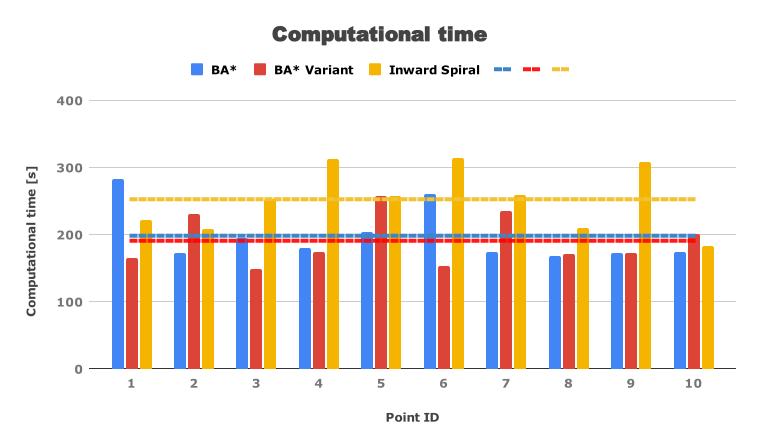
\includegraphics[width=0.99\textwidth]{figures/Computational time.pdf}
%     \caption{Results of Experiment 2. Computational time to generate a path that reaches the goal coverage for each algorithm. The horizontal dotted lines represent the average value of the corresponding algorithm.}
%     \label{fig:computational_time}
% \end{figure}

% \section{Experiment 3 - Sampled BA* \& Spiral}

% The same coverage goal was used in experiment 3 as in experiment 2. The parameters of the Sampled BA* \& Spiral algorithm were hand tuned to keep the computational time close to the times in experiment 2, see figure \ref{fig:exp3_computational_time} while minimizing the length of the path and the total rotation. 

% In figures \ref{fig:exp3_length_of_path} and \ref{fig:exp3_total_rotation} the Sampled BA* and Spiral is compared with the results of BA* and BA* variant in experiment 2.

% \begin{figure}
%     \centering
%     \includegraphics[width=0.99\textwidth]{figures/Computational time(1).pdf}
%     \caption{Results of Experiment 3. Shows that  computational times of the Sampled BA* & Spiral is close to the computational times of the other algorithms in experiment 2. The horizontal dotted lines represent the average value of the corresponding algorithm.}
%     \label{fig:exp3_computational_time}
% \end{figure}


% \begin{figure}
%     \centering
%     \includegraphics[width=0.99\textwidth]{figures/Length of path(1).pdf}
%     \caption{Results of Experiment 3. The length of the generated paths. The horizontal dotted lines represent the average value of the corresponding algorithm.}
%     \label{fig:exp3_length_of_path}
% \end{figure}


% \begin{figure}
%     \centering
%     \includegraphics[width=0.99\textwidth]{figures/Total Rotation(1).pdf}
%     \caption{Results of Experiment 3. The total rotation of the paths. The horizontal dotted lines represent the average value of the corresponding algorithm.}
%     \label{fig:exp3_total_rotation}
% \end{figure}





% This chapter presents the results. Note that the results are presented
% factually, striving for objectivity as far as possible.  The results
% shall not be analyzed, discussed or evaluated.  This is left for the
% discussion chapter.

% In case the method chapter has been divided into subheadings such as
% pre-study, implementation and evaluation, the result chapter should
% have the same sub-headings. This gives a clear structure and makes the
% chapter easier to write.

% In case results are presented from a process (e.g. an implementation
% process), the main decisions made during the process must be clearly
% presented and justified. Normally, alternative attempts, etc, have
% already been described in the theory chapter, making it possible to
% refer to it as part of the justification.

%%%%%%%%%%%%%%%%%%%%%%%%%%%%%%%%%%%%%%%%%%%%%%%%%%%%%%%%%%%%%%%%%%%%%%
%%% lorem.tex ends here

%%% Local Variables: 
%%% mode: latex
%%% TeX-master: "demothesis"
%%% End: 

\include{8-discussion}
\include{9-conclusion}
\printbibliography

\end{document}

%%%%%%%%%%%%%%%%%%%%%%%%%%%%%%%%%%%%%%%%%%%%%%%%%%%%%%%%%%%%%%%%%%%%%%
%%% demothesis.tex ends here

